% === CONTEXTO === %

\vspace{2em}
\subsection{Contexto} 

En el análisis de redes sociales, una \textit{ego-network} \cite{Leskovec} es una red compuesta por las amistades que existen entre los amigos de un individuo, el `ego'. Estas redes son centrales en aplicaciones como Facebook, Google+ o Twitter. 

\vspace{1em}
En particular, dada una red de estas características, resulta de interés poder identificar los círculos sociales ---conjuntos, disjuntos y anidados--- a los que pertenece un usuario. Leskovec \cite{Leskovec} propone un método de aprendizaje no supervisado para lograr inferirlos, que se nutre de la siguiente información: un grafo \textbf{E} (la red) ---donde se espera que exista una correlación fuerte entre un círculo y la densidad de conexiones entre los nodos que lo componen--- y un conjunto de atributos \textbf{C} para cada nodo ---donde se espera que exista una correlación entre un círculo y la similaridad de los atributos de los nodos que lo componen---.

\vspace{1em}
\begin{figure}[!htbp]
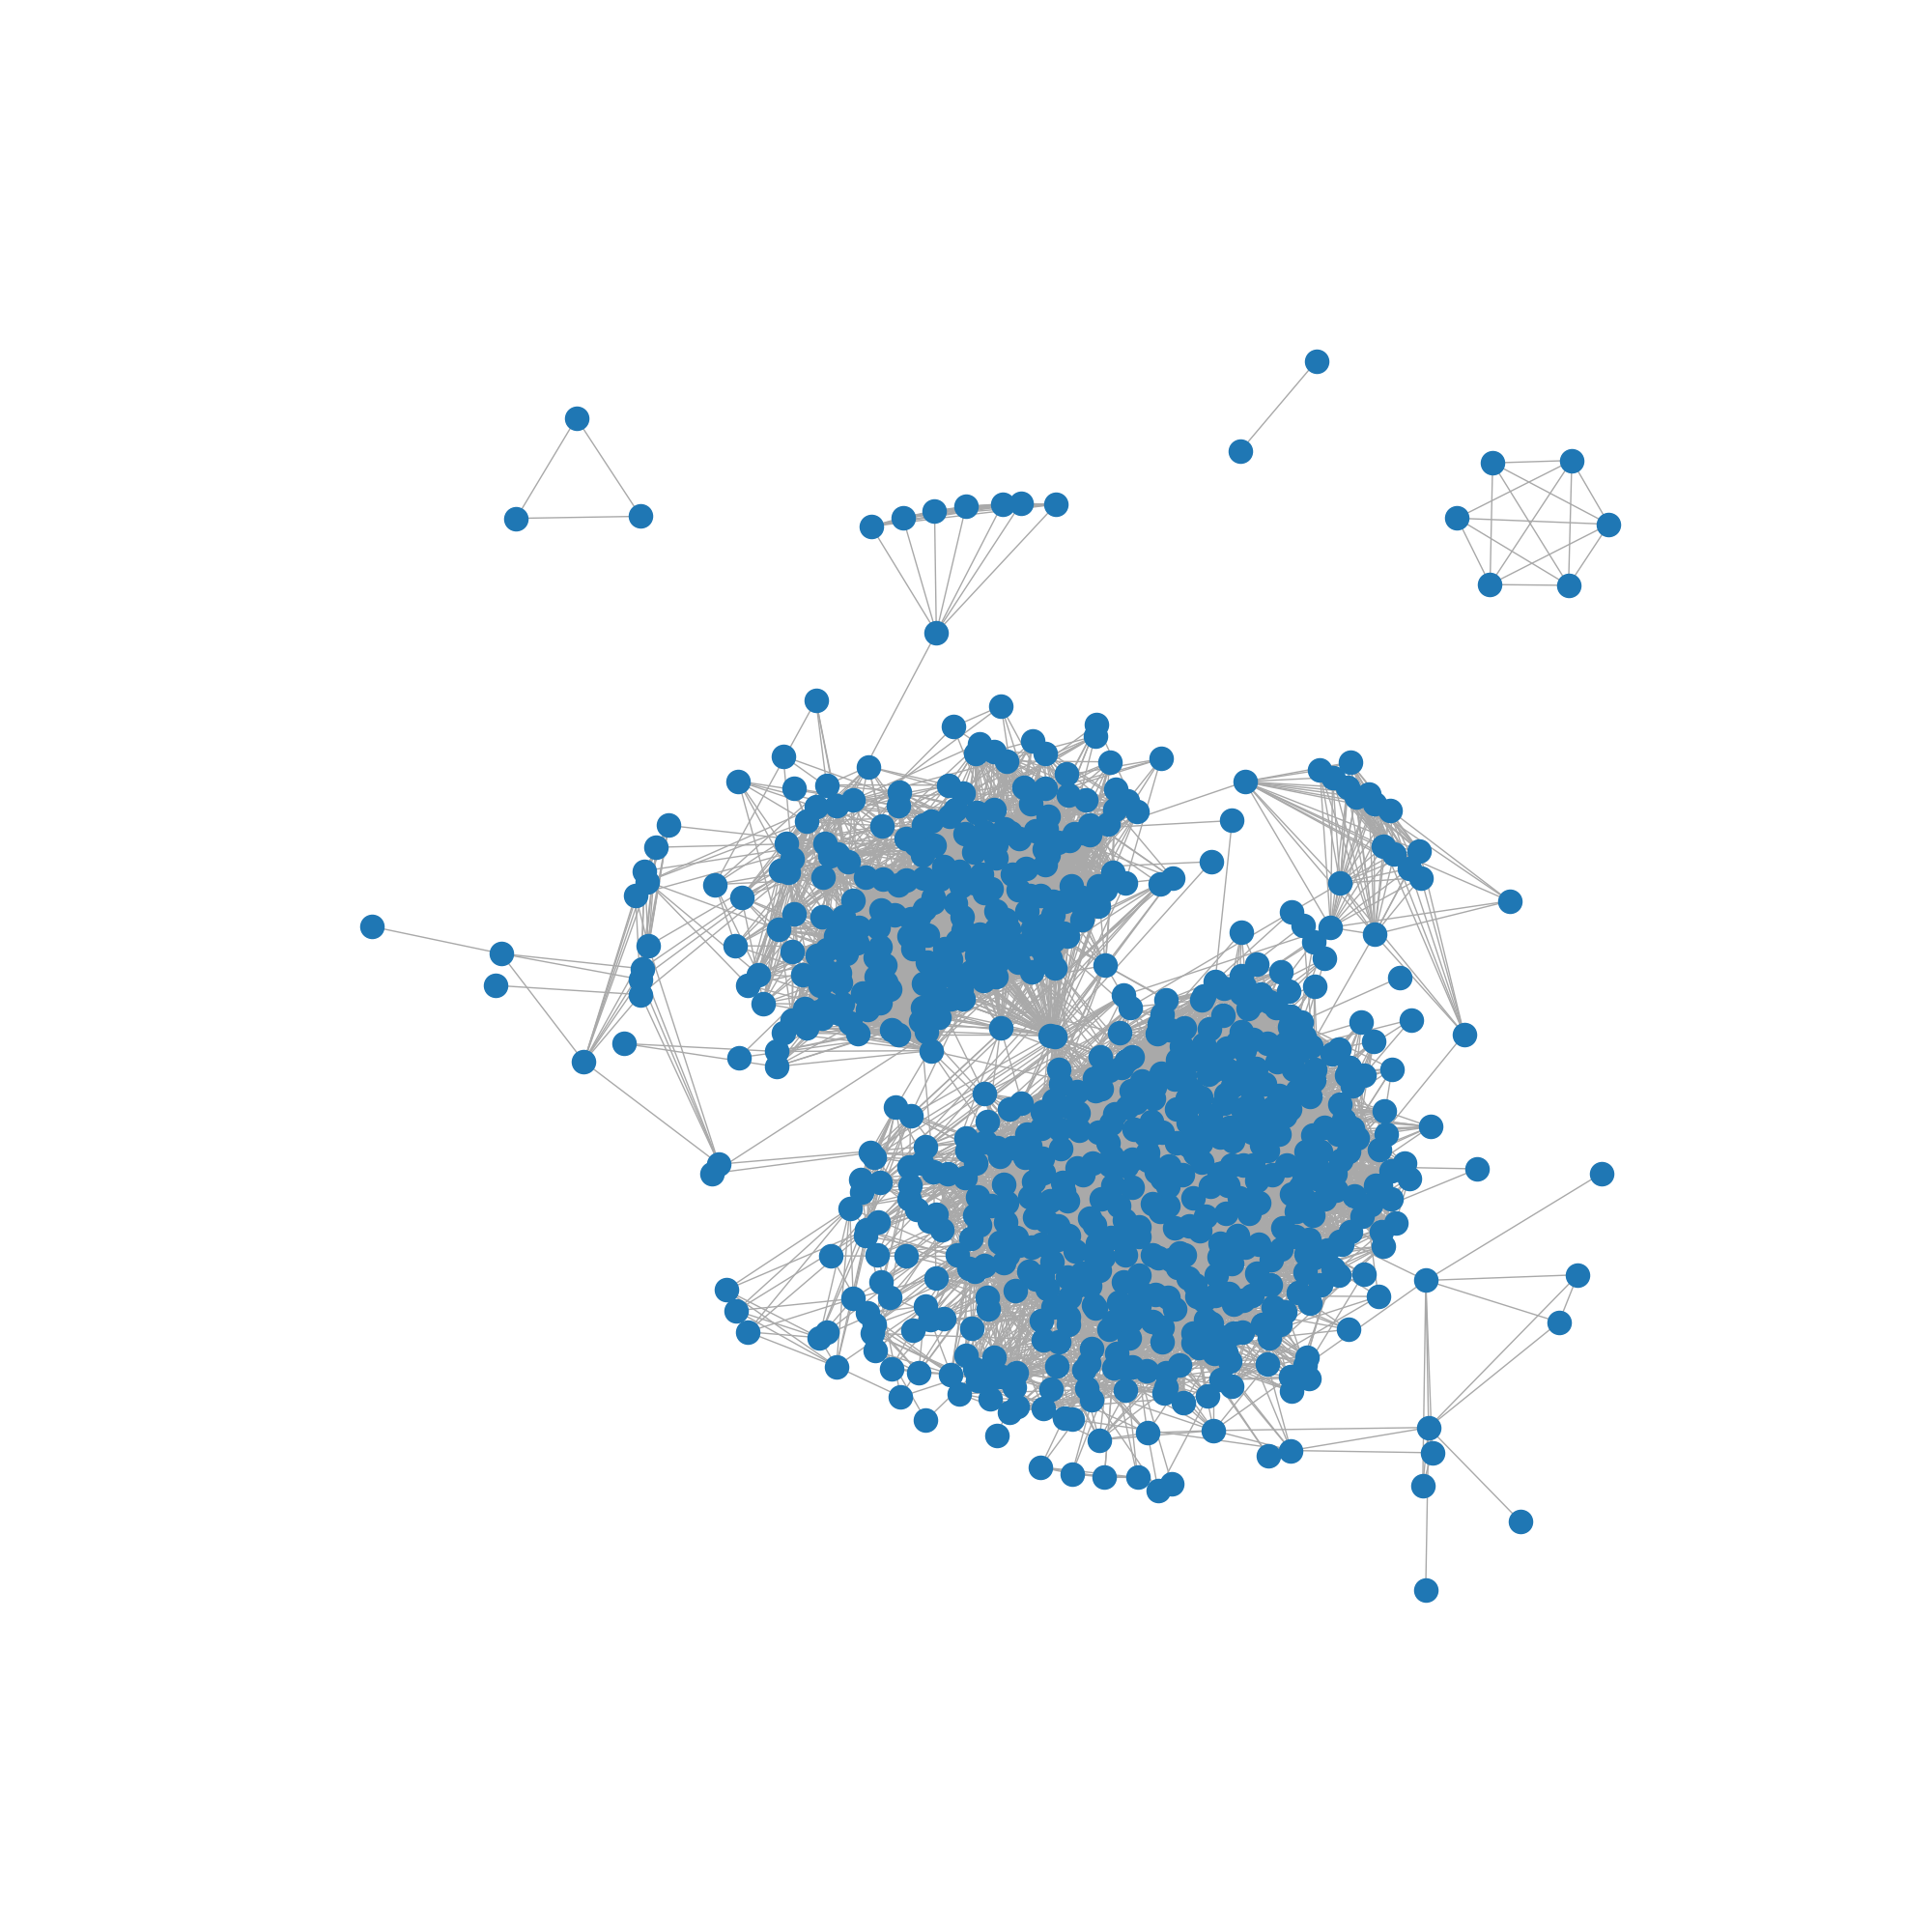
\includegraphics[scale=0.25, trim=200 200 200 200, clip]{/files/src/.media/ego/grafo_facebook.png}
\caption{Una \textit{ego-network} de Facebook compuesta por 786 nodos. Cada vértice representa un individuo, cada arista la existencia de una amistad.} \label{ego_facebook}
\end{figure}

\vspace{1em}
En este análisis\footnote{El script asociado se puede encontrar en \textit{./experimentos/ego\_facebook.py}, los archivos con los resultados  en \textit{./experimentos/resultados/ego-facebook/}.} estimaremos la red `ego' \textbf{E} de la figura (\ref{ego_facebook}.), por medio de la construcción de una matriz de similaridad que utilice el conjunto de atributos \textbf{C} asociados a \textbf{E}\footnote{Por cuestiones de privacidad, los datos están despojados de cualquier referencia a sus cualidades: los nodos y atributos se distinguen por medio de números; los atributos, además, por una parametrización binaria que designa si el nodo porta o no cierta cualidad.}. También, buscaremos reducir su dimensionalidad por medio del análisis de componentes principales.




% === SIMILARIDAD @ ATRIBUTOS === %

\vspace{2em}
\subsection{Matriz de similaridad}

%Queremos generar una aproximación de nuestra red `ego' original \textbf{E} en base a los atributos en \textbf{C} de los usuarios que la componen. Es decir, buscamos un método que nos permita comparar los atributos de dos nodos diferentes y, bajo algún criterio propuesto, conectarlos o no en fin de replicar nuestra red verdadera. 

Queremos generar una aproximación de nuestra red `ego' original, \textbf{E}, a partir de los atributos de los usuarios que la componen, definidos en \textbf{C}. Es decir, buscamos un método que nos permita comparar los atributos de dos nodos diferentes y, bajo algún criterio propuesto, decidir conectarlos o no con el fin de replicar la red verdadera. 

% Intuitivamente, una forma de adivinar si dos usuarios se encuentran conectados en una red es contando la cantidad de atributos que comparten. Se podría pensar que si coinciden en muchos existe una mayor probabilidad de que pertenezcan al mismo círculo, mientras que sino podría ser que ni siquiera se conozcan. Las estructuras que utilizaremos para replicar esta línea de pensamiento son las \textit{matrices de similaridad}, las cuales dado un conjunto de datos $X$ aplican una función a cada par de datos $ij$.

\vspace{1em}
Intuitivamente, una forma de decidir si dos usuarios deberían estar conectados, o no, es contar la cantidad de atributos que comparten. Se podría pensar que si coinciden en muchos, entonces existe una mayor probabilidad que pertenezcan al mismo círculo. Otra forma podría ser medir la distancia, a partir de alguna norma, entre sus vectores de atributos.%Sino, podría ser que ni siquiera se conozcan. 

%\vspace{1em}
%Para replicar esta línea de pensamiento, utilizaremos 
De manera general, podemos pensar en las \textit{matrices de similaridad}. Dado un conjunto de datos $X$, se aplica una función a cada par de elementos $x_i$, $x_j$ tal que:

\vspace{1em}
\begin{equation}
    s_{ij} = f(x_i, x_j)
\end{equation}

%Nuestra tabla de atributos\footnote{La misma puede encontrarse en \textit{./catedra/ego-facebook.feat}.} es tal que la primera columna contiene los tags correspondientes a cada usuario, y el resto de las columnas forman \textbf{C}, donde la $fila_i(\textbf{C})$ son los atributos del usuario $tag_i$. Tomemos entonces nuestra matriz de similaridad $\textbf{S} = \textbf{CC}^{t}$, tal que $\textbf{S}_{ij}$ expresa la similaridad entre la $tag_{i}$ y $tag_{j}$ computando el producto interno de sus respectivos atributos. Con esta información podemos luego proponer diferentes umbrales $u$ entre el menor y mayor valor en \textbf{S}, y establecer que $\textbf{S}_{ij} > u$ indica que los $tag_{i}$ y $tag_{j}$ están conectados en nuestra aproximación. 

\vspace{2em}
En nuestro caso, trabajaremos con una tabla de atributos\footnote{La misma se puede encontrar en \textit{./catedra/ego-facebook.feat}. Dado que la red original y esta tabla no comparten todos sus nodos, se realizó un proceso de filtrado y limpieza. Las versiones corregidas se encuentran en \textit{./experimentos/resultados/ego-facebook/}.} cuya primer columna contiene las etiquetas ($tags$) de cada nodo en la red, y el resto de las columnas forman \textbf{C} ---donde la $\text{\textit{fila}}_i(\textbf{C})$ representa los atributos del usuario definido por la etiqueta $i$---. A partir de estos datos, definiremos la matriz de similaridad de la siguiente forma:

\vspace{1em}
\begin{equation}
    \mathbf{S} = \mathbf{C}\ \mathbf{C}^{t}
\end{equation}

\vspace{1em}
\noindent donde $s_{ij}$ expresa la similaridad entre el nodo $i$ y el $j$ por medio del producto interno de sus respectivos vectores de atributos. 

\vspace{1em}
Con esta información propondremos diferentes umbrales $u$ en el rango $[min(\mathbf{S}),\ max(\mathbf{S}))$ que servirán como criterio para aproximar \textbf{E}. Si $s_{ij} > u$, entonces los nodos $i$ y $j$ estarán conectados. 

%Procedemos a mostrar los resultados obtenidos. Tomando $u \in [min{\textbf{S}_{ij}},\ max{\textbf{S}_{ij}}) = [0, 22)$, $u \in \mathbb{Z}$, obtuvimos 22 diferentes aproximaciones de \textbf{E}.

\vspace{2em}
\noindent \textsc{Resultados}. Vemos que cada elemento $s_{ij}$ es entero, por producto punto de enteros, y $[min(\mathbf{S}),\ max(\mathbf{S})) = [0, 22)$. A partir de estas observaciones aproximamos \textbf{E} por medio de 22 umbrales distintos: $[0,\ 1,\ ...,\ 22]$. La figura (\ref{grafos_aproximados}.) muestra una representación de los grafos obtenidos más significativos. 

%Obsérvese que cuanto más alto sea el umbral, menores conexiones tendremos en nuestro grafo aproximado. En particular, con $u = 0$ se obtiene un grafo donde todos los usuarios están conectados entre sí, y con $u > 12$ grafos con ninguna arista. Nos enfocaremos entonces con los asociados a $u \in [0, 12]$, ya que son los que revelan información de interés.

\vspace{1em}
Observamos que cuanto mayor sea el umbral, menos conexiones tendremos en nuestra aproximación. En particular, con $u = 0$ se obtiene un grafo donde casi todos los usuarios están conectados entre sí, y con $u > 12$ obtenemos un grafo sin ninguna arista. Nos enfocaremos entonces en los grafos asociados a $u \in [0, 12]$, ya que estos son los que revelan la mayor cantidad de información. 

\vspace{1em}
\begin{figure}[!htbp]
    \centering
    \subfloat[$u = 0$]{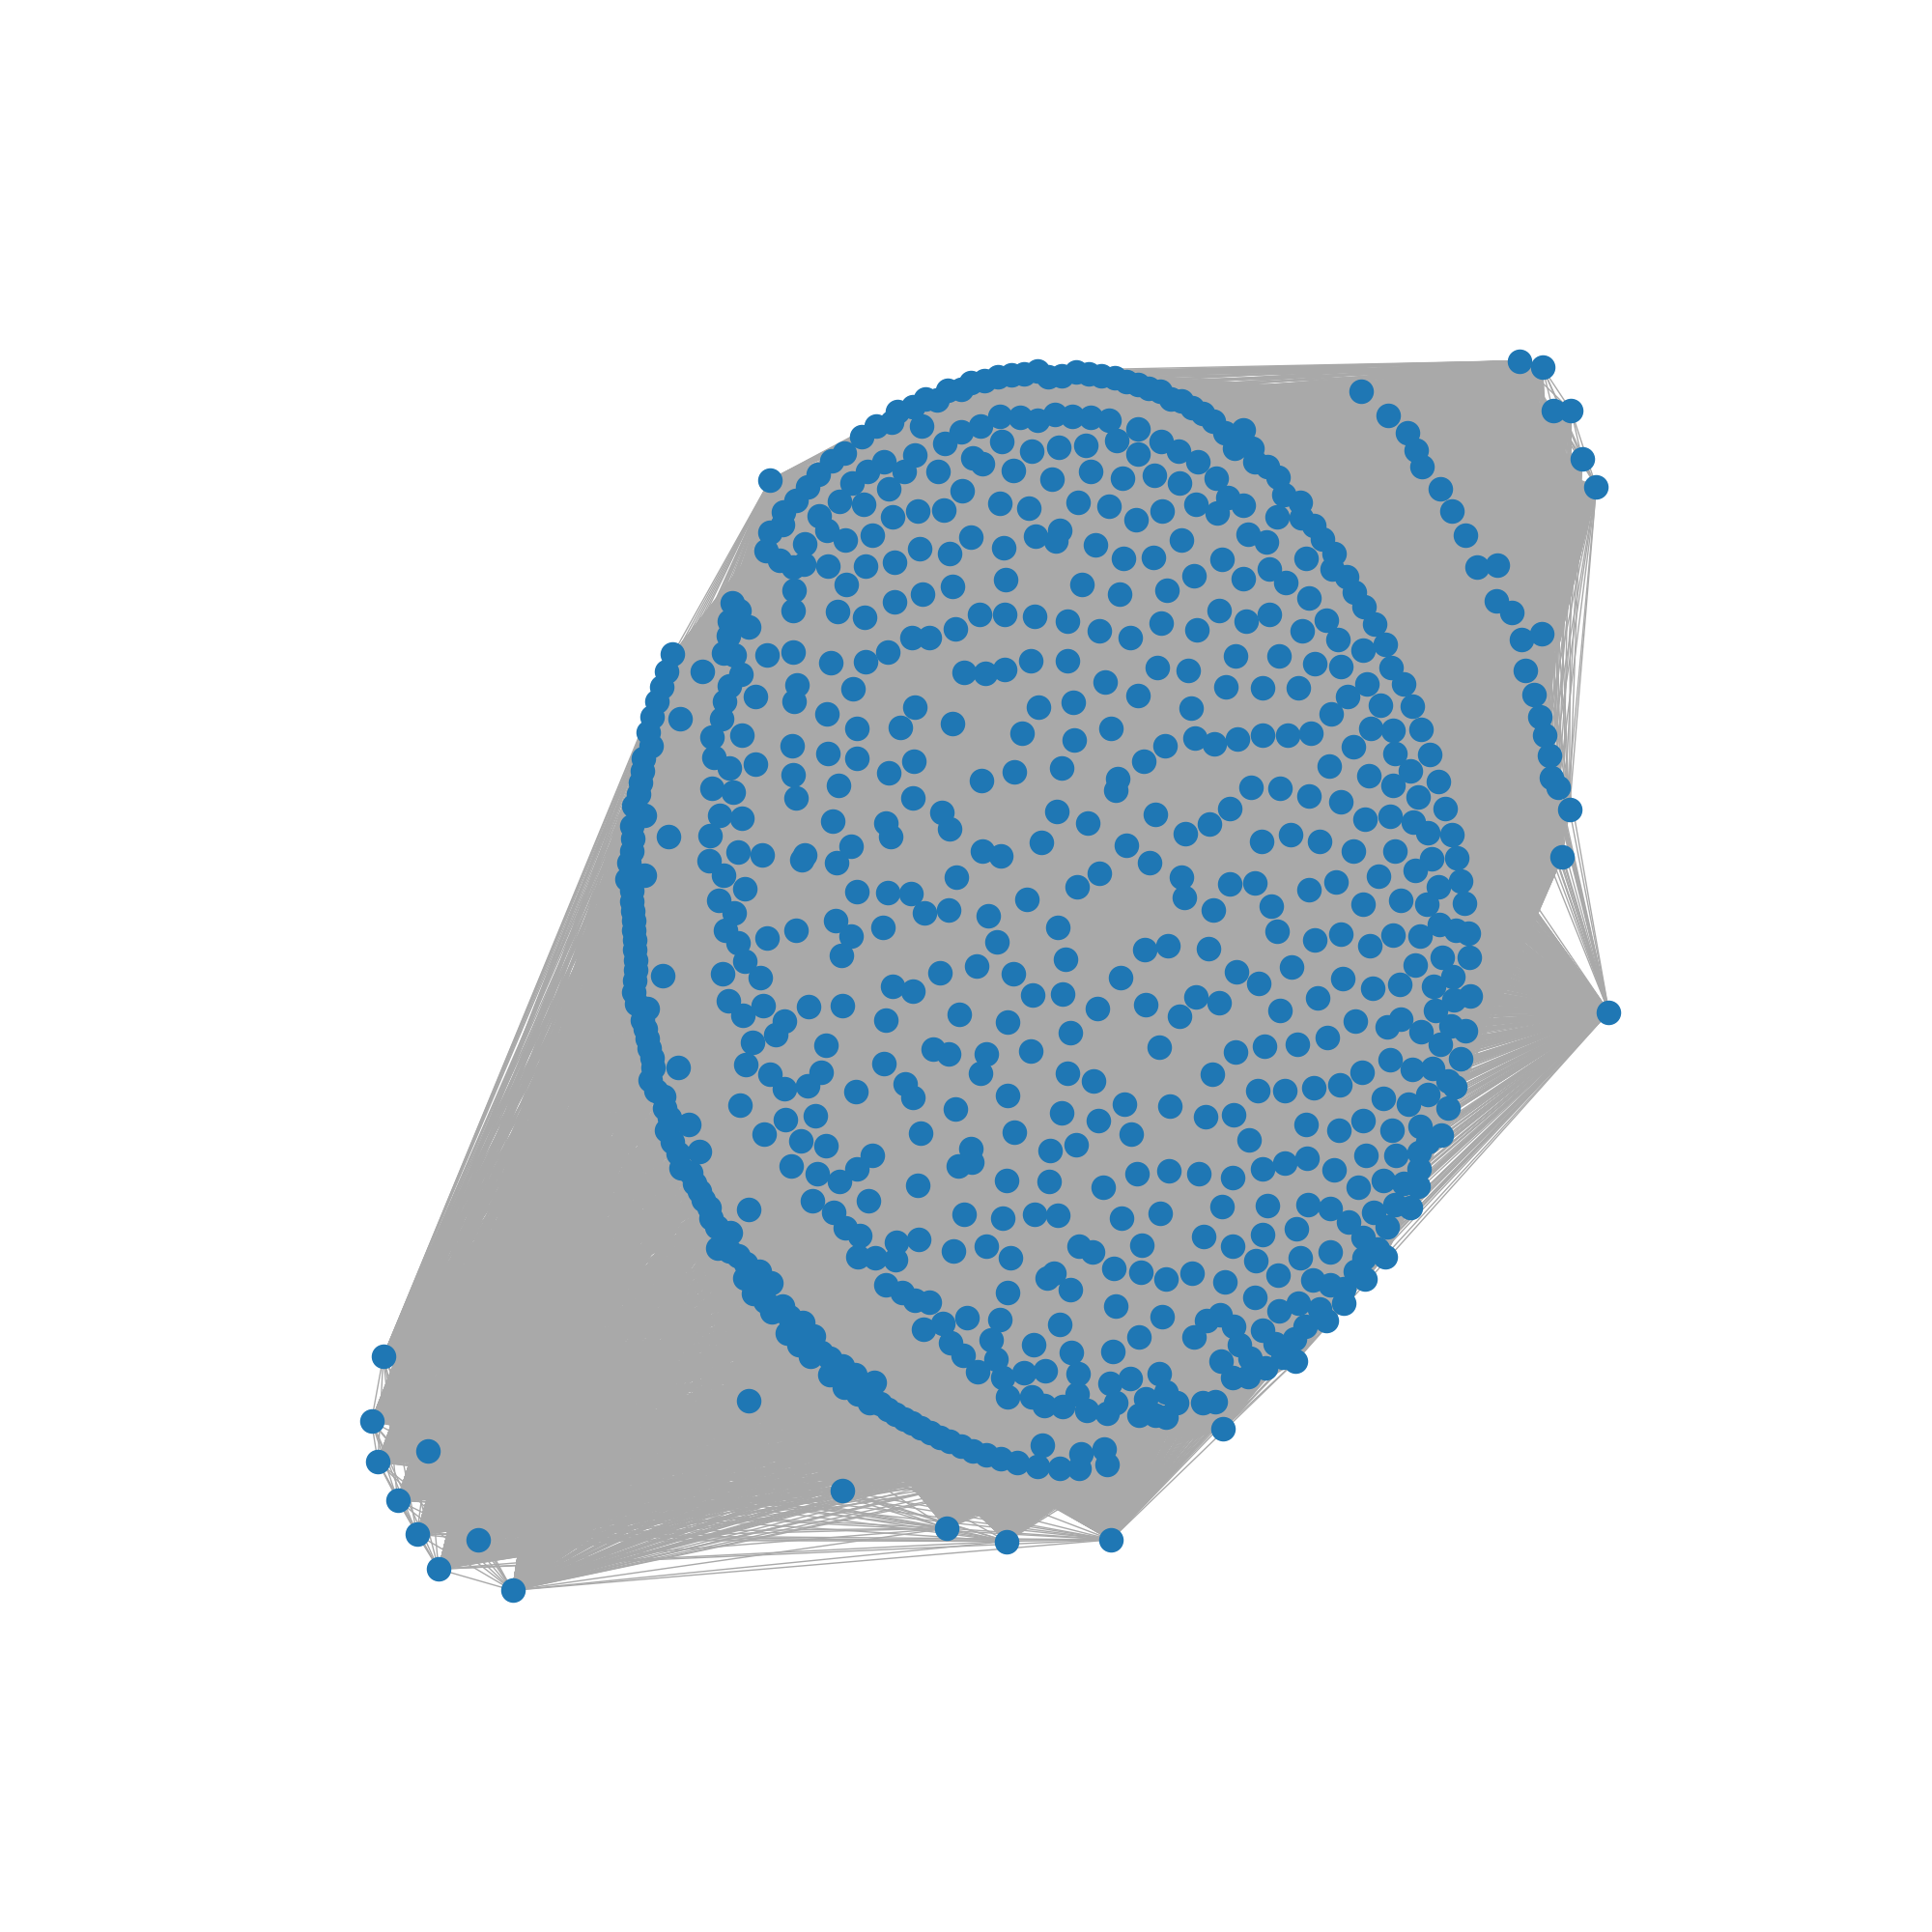
\includegraphics[width=.25\textwidth]{/files/src/.media/ego/grafo_1.png}}\hfill
    \subfloat[$u = 1$]{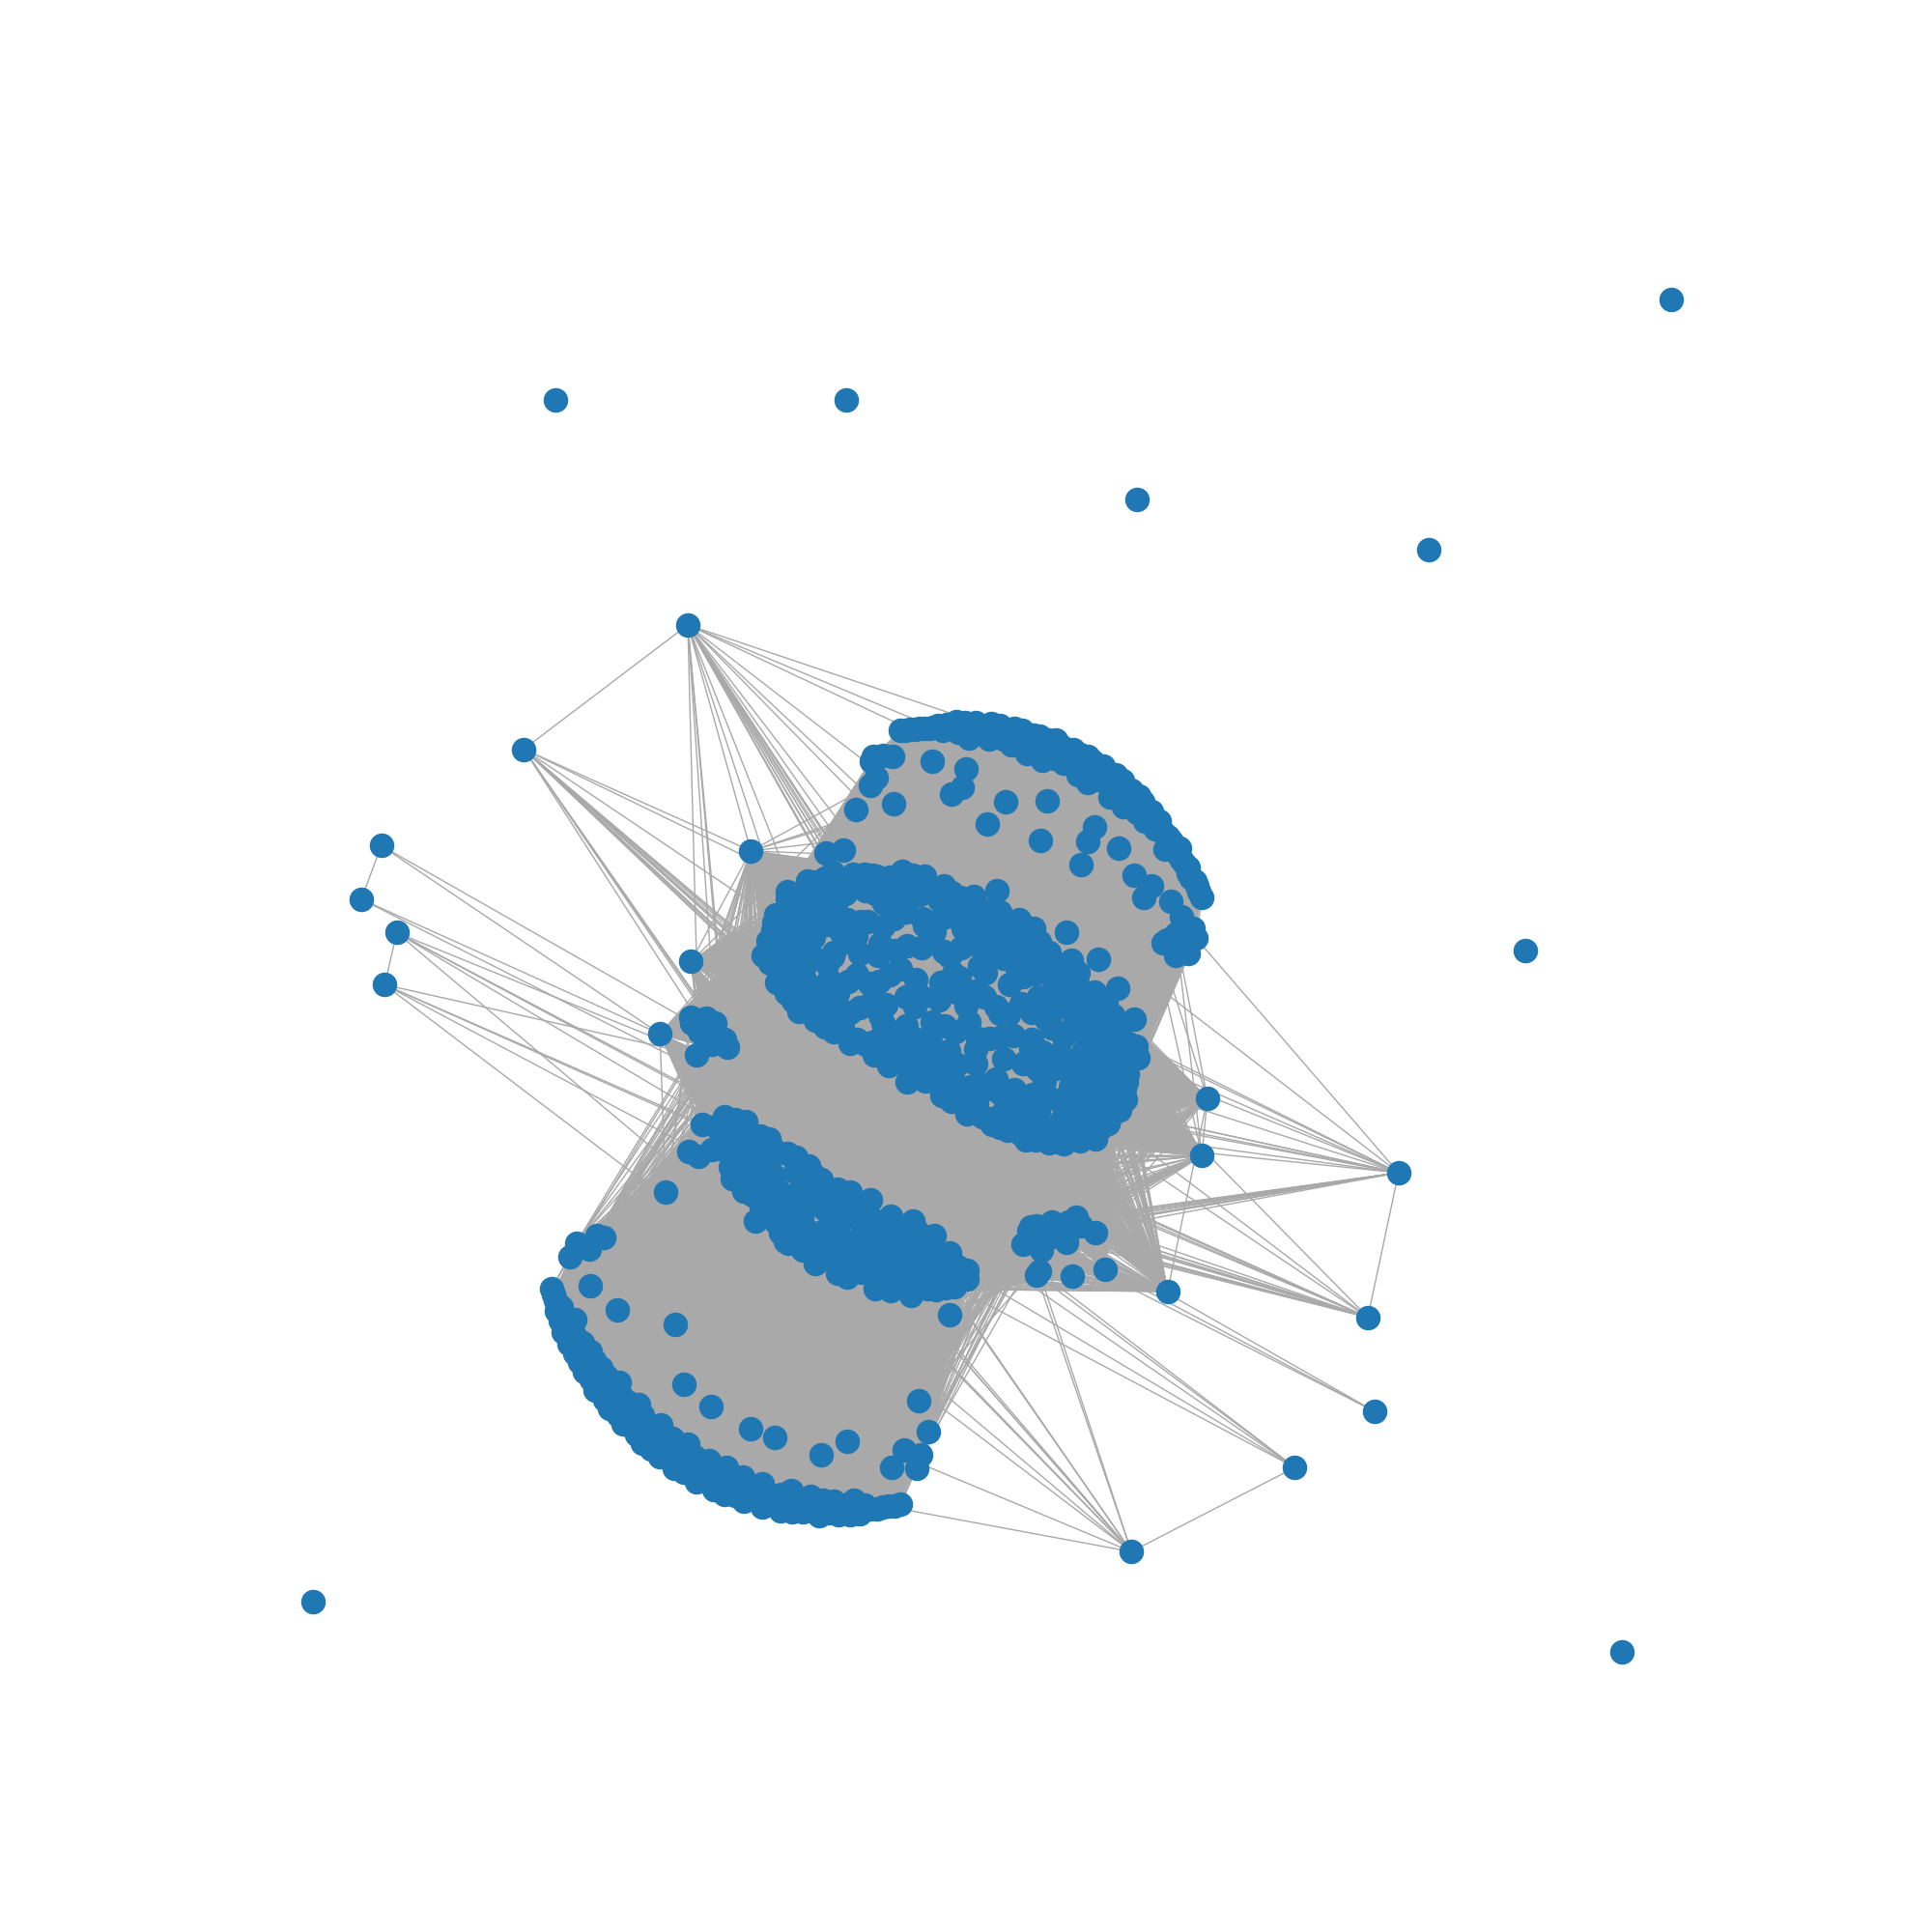
\includegraphics[width=.25\textwidth]{/files/src/.media/ego/grafo_2.png}}\hfill
    \subfloat[$u = 2$]{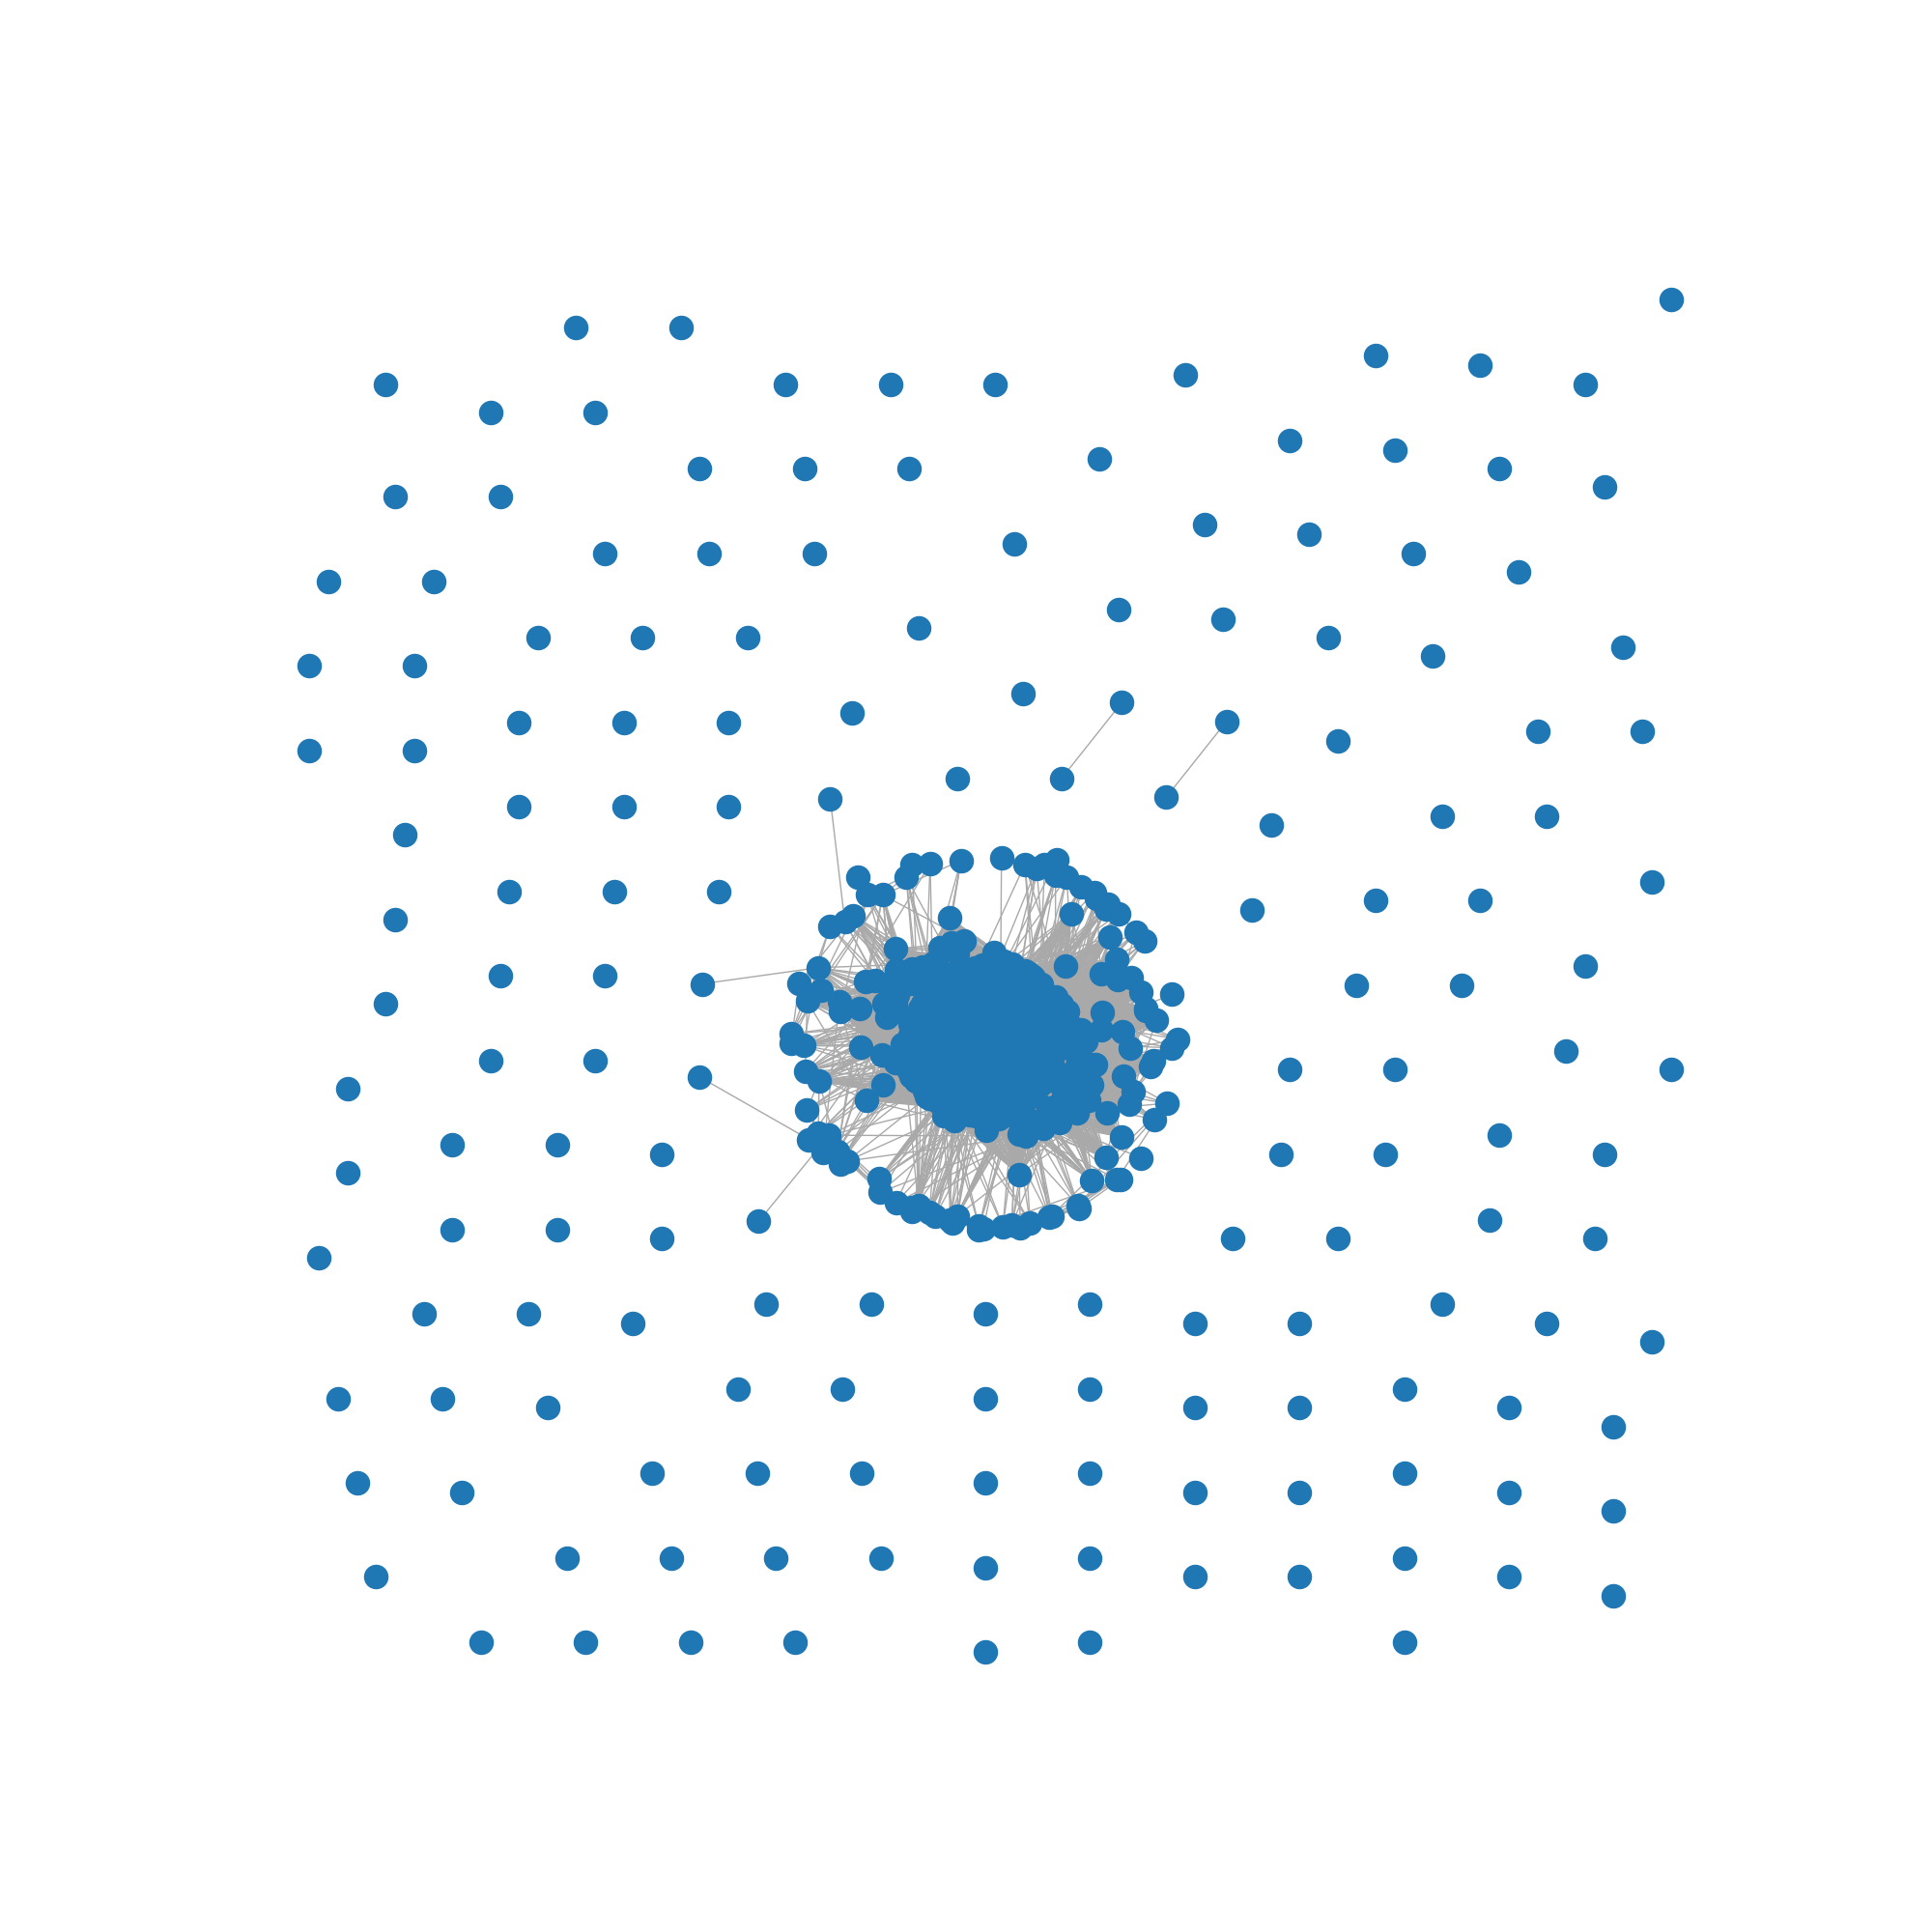
\includegraphics[width=.25\textwidth]{/files/src/.media/ego/grafo_3.png}}\hfill
    \subfloat[$u = 3$]{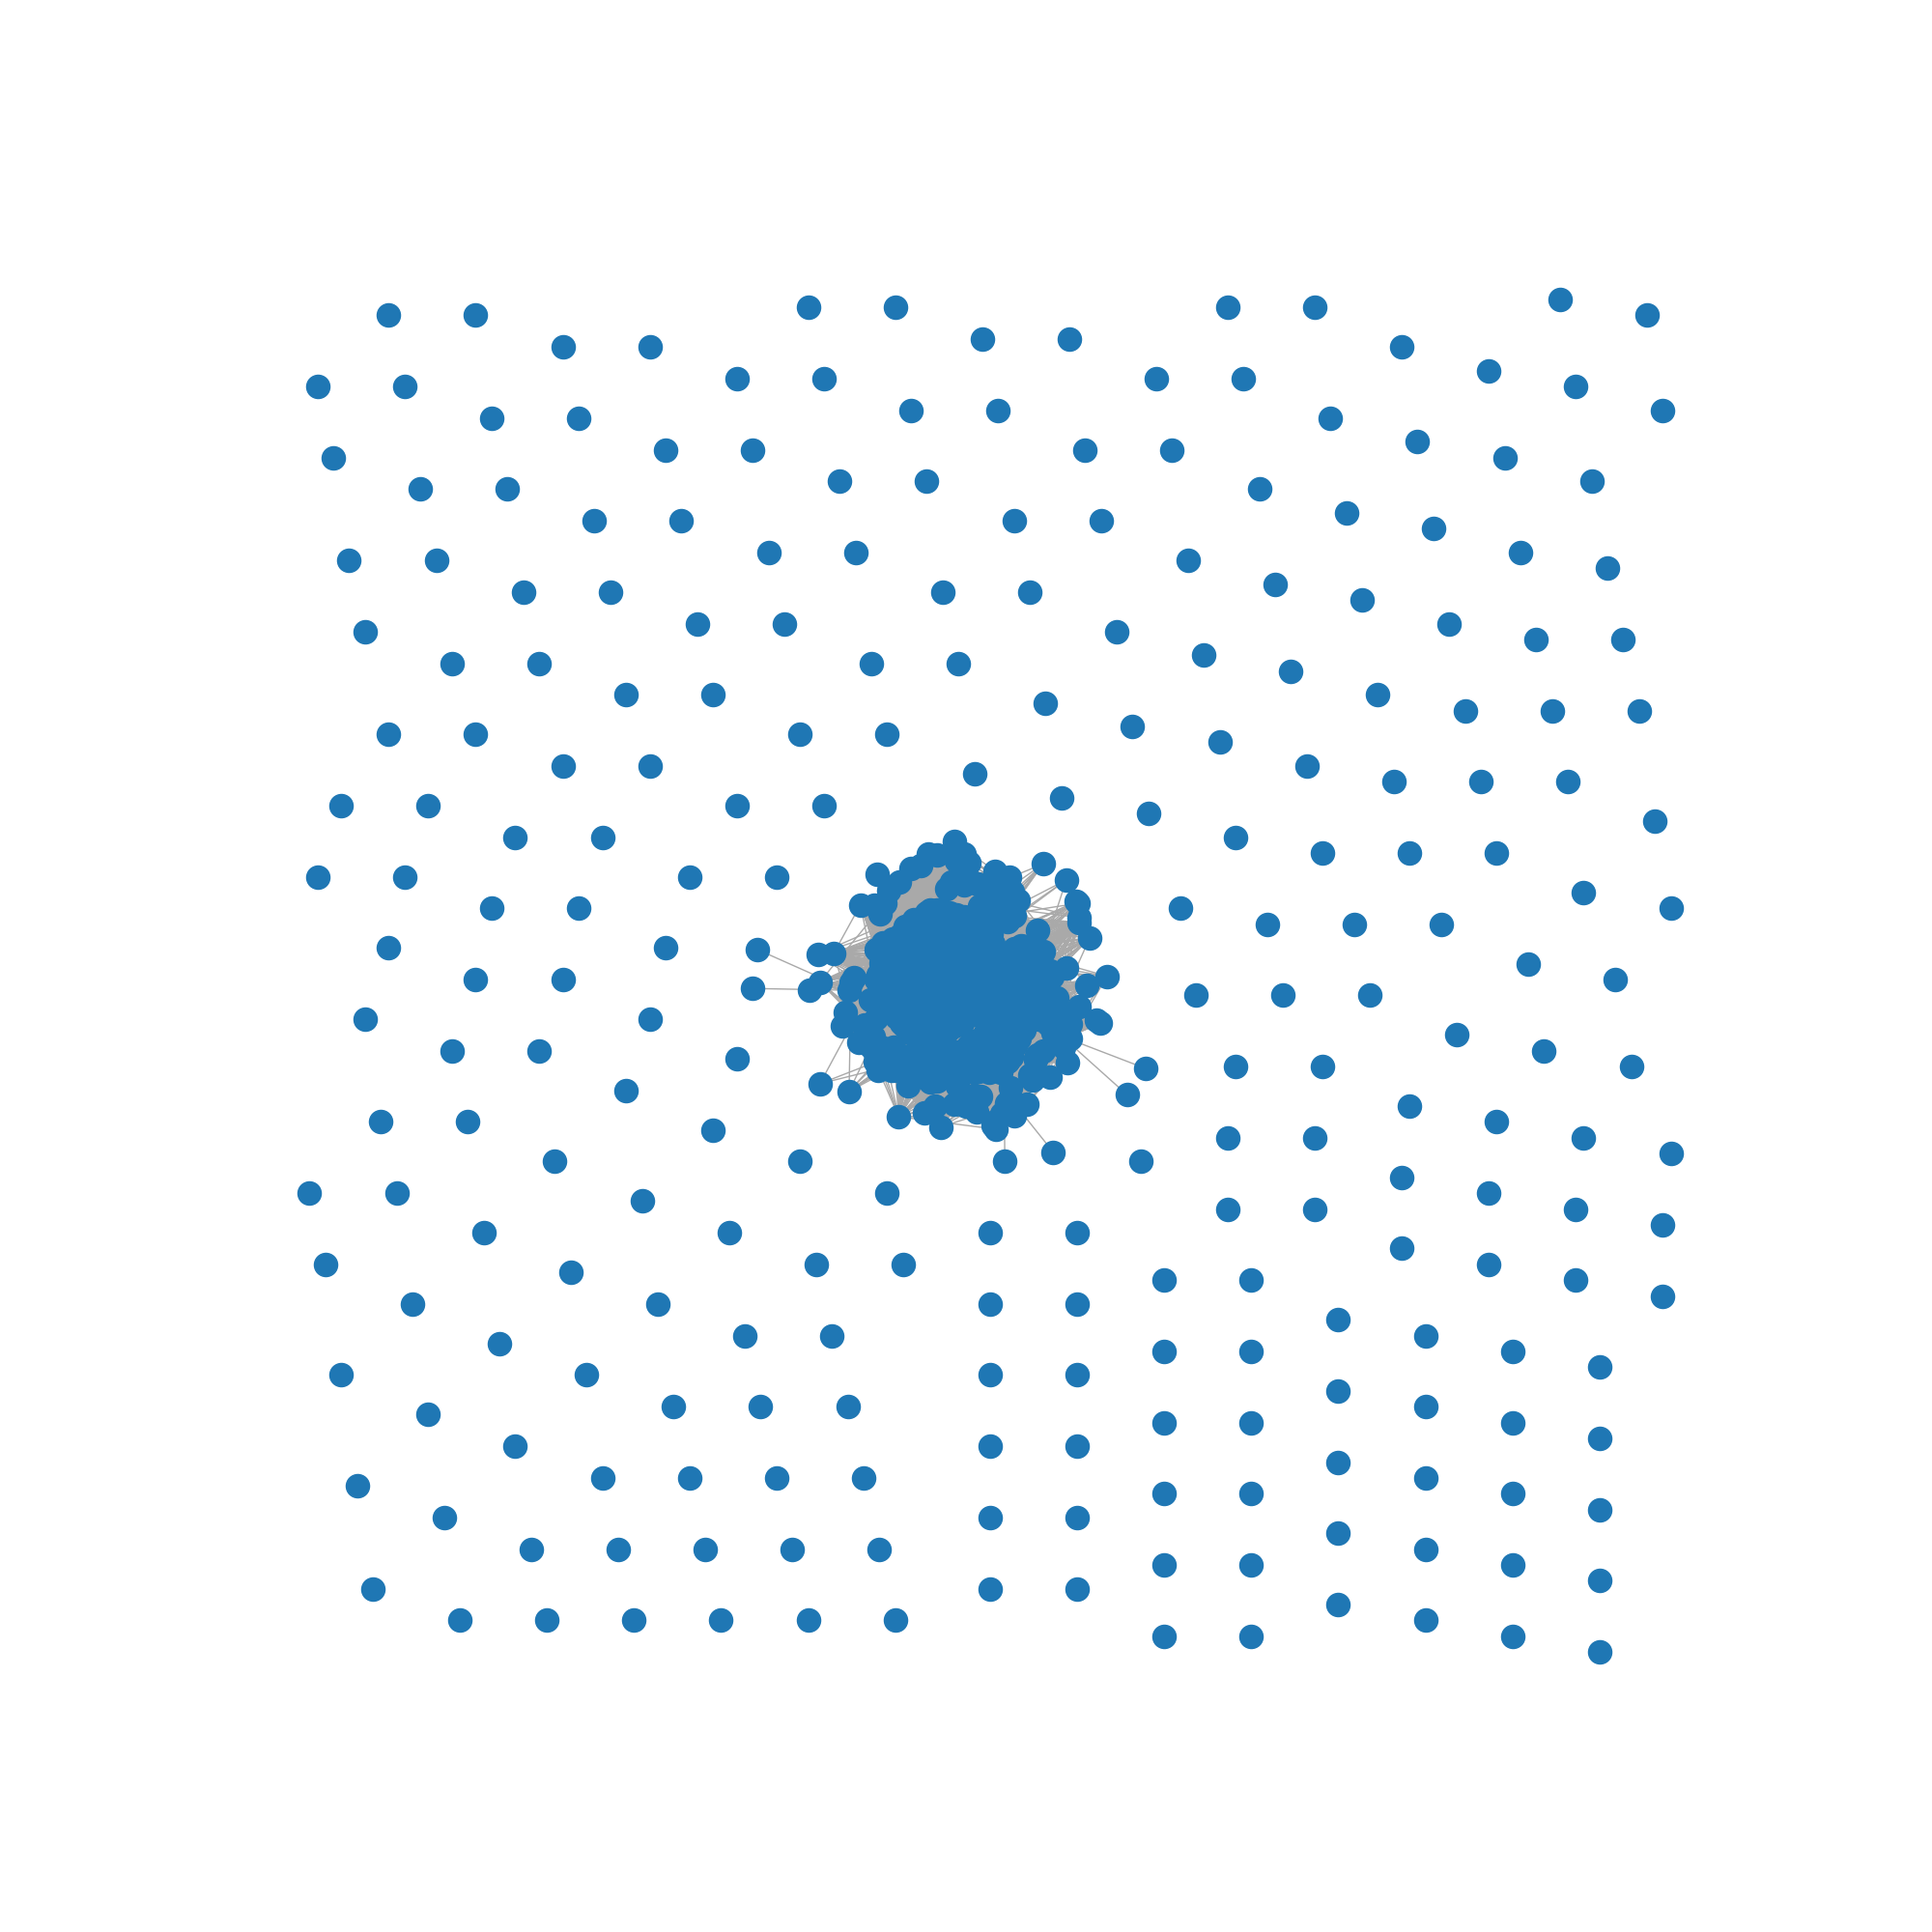
\includegraphics[width=.25\textwidth]{/files/src/.media/ego/grafo_4.png}}\hfill
% \end{figure}
% \begin{figure}[!htbp]
%     \ContinuedFloat
%     \centering
    \\[\smallskipamount]
    \subfloat[$u = 4$]{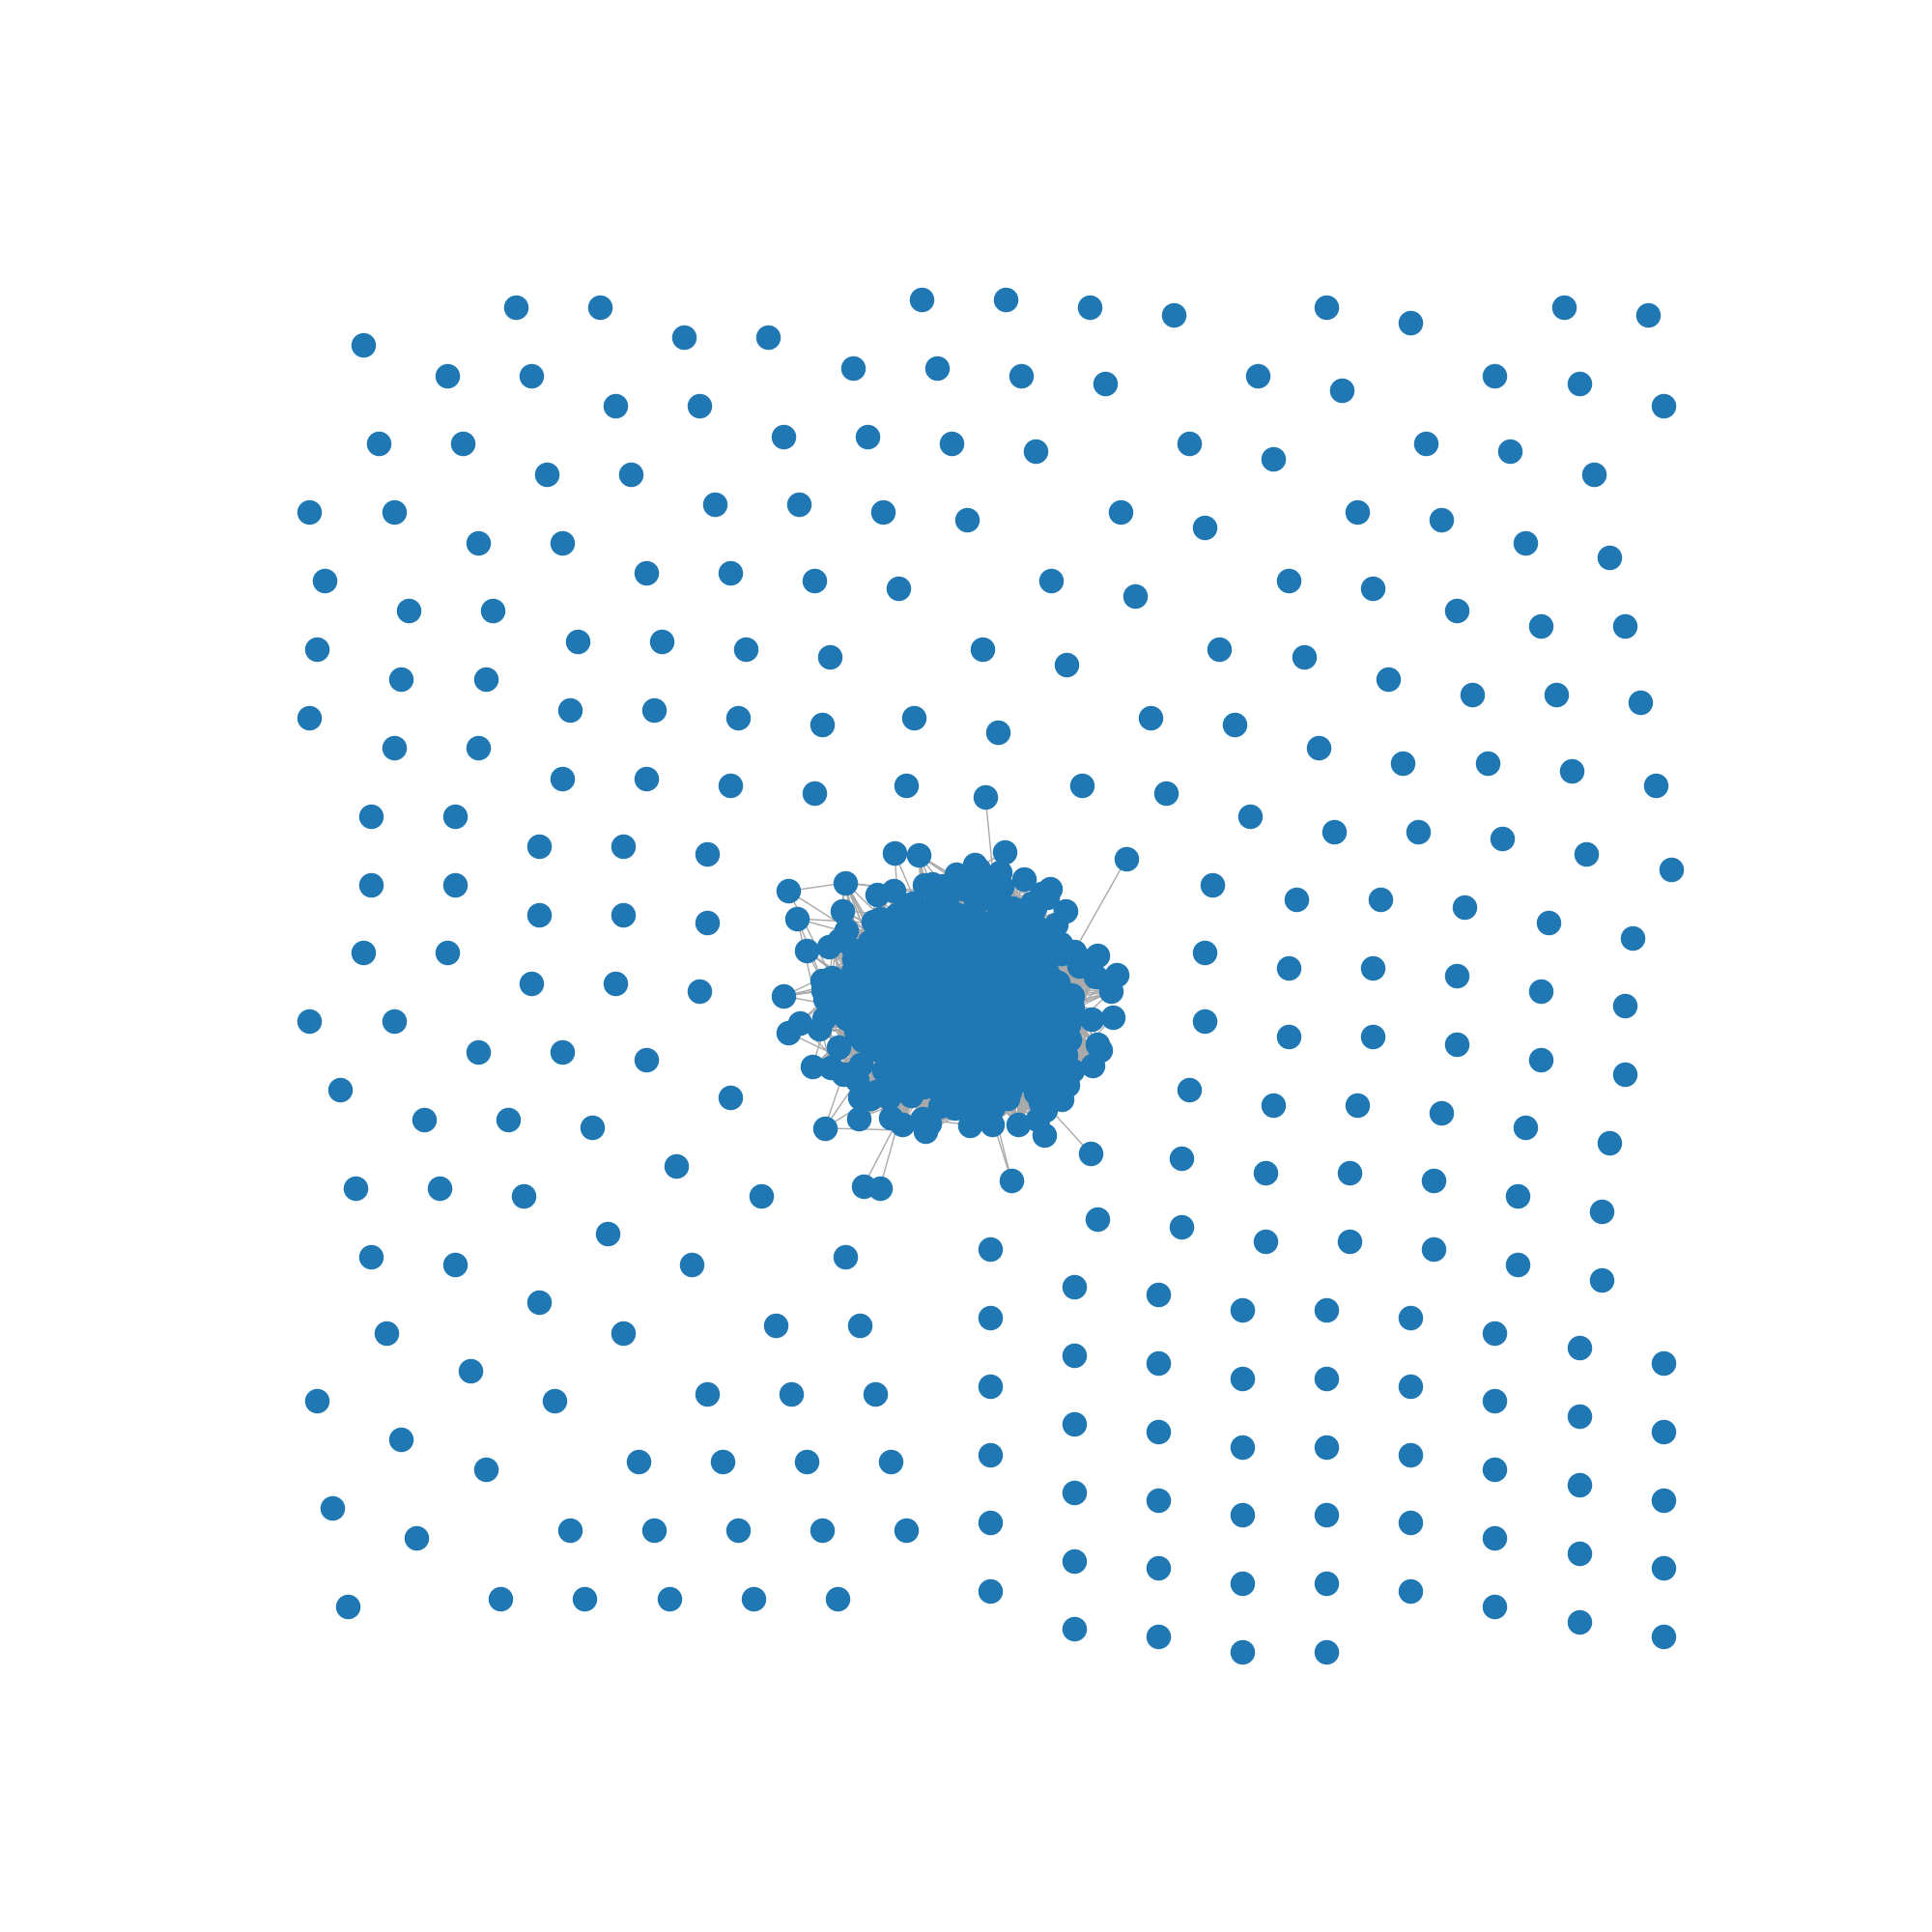
\includegraphics[width=.25\textwidth]{/files/src/.media/ego/grafo_5.png}}\hfill
    \subfloat[$u = 5$]{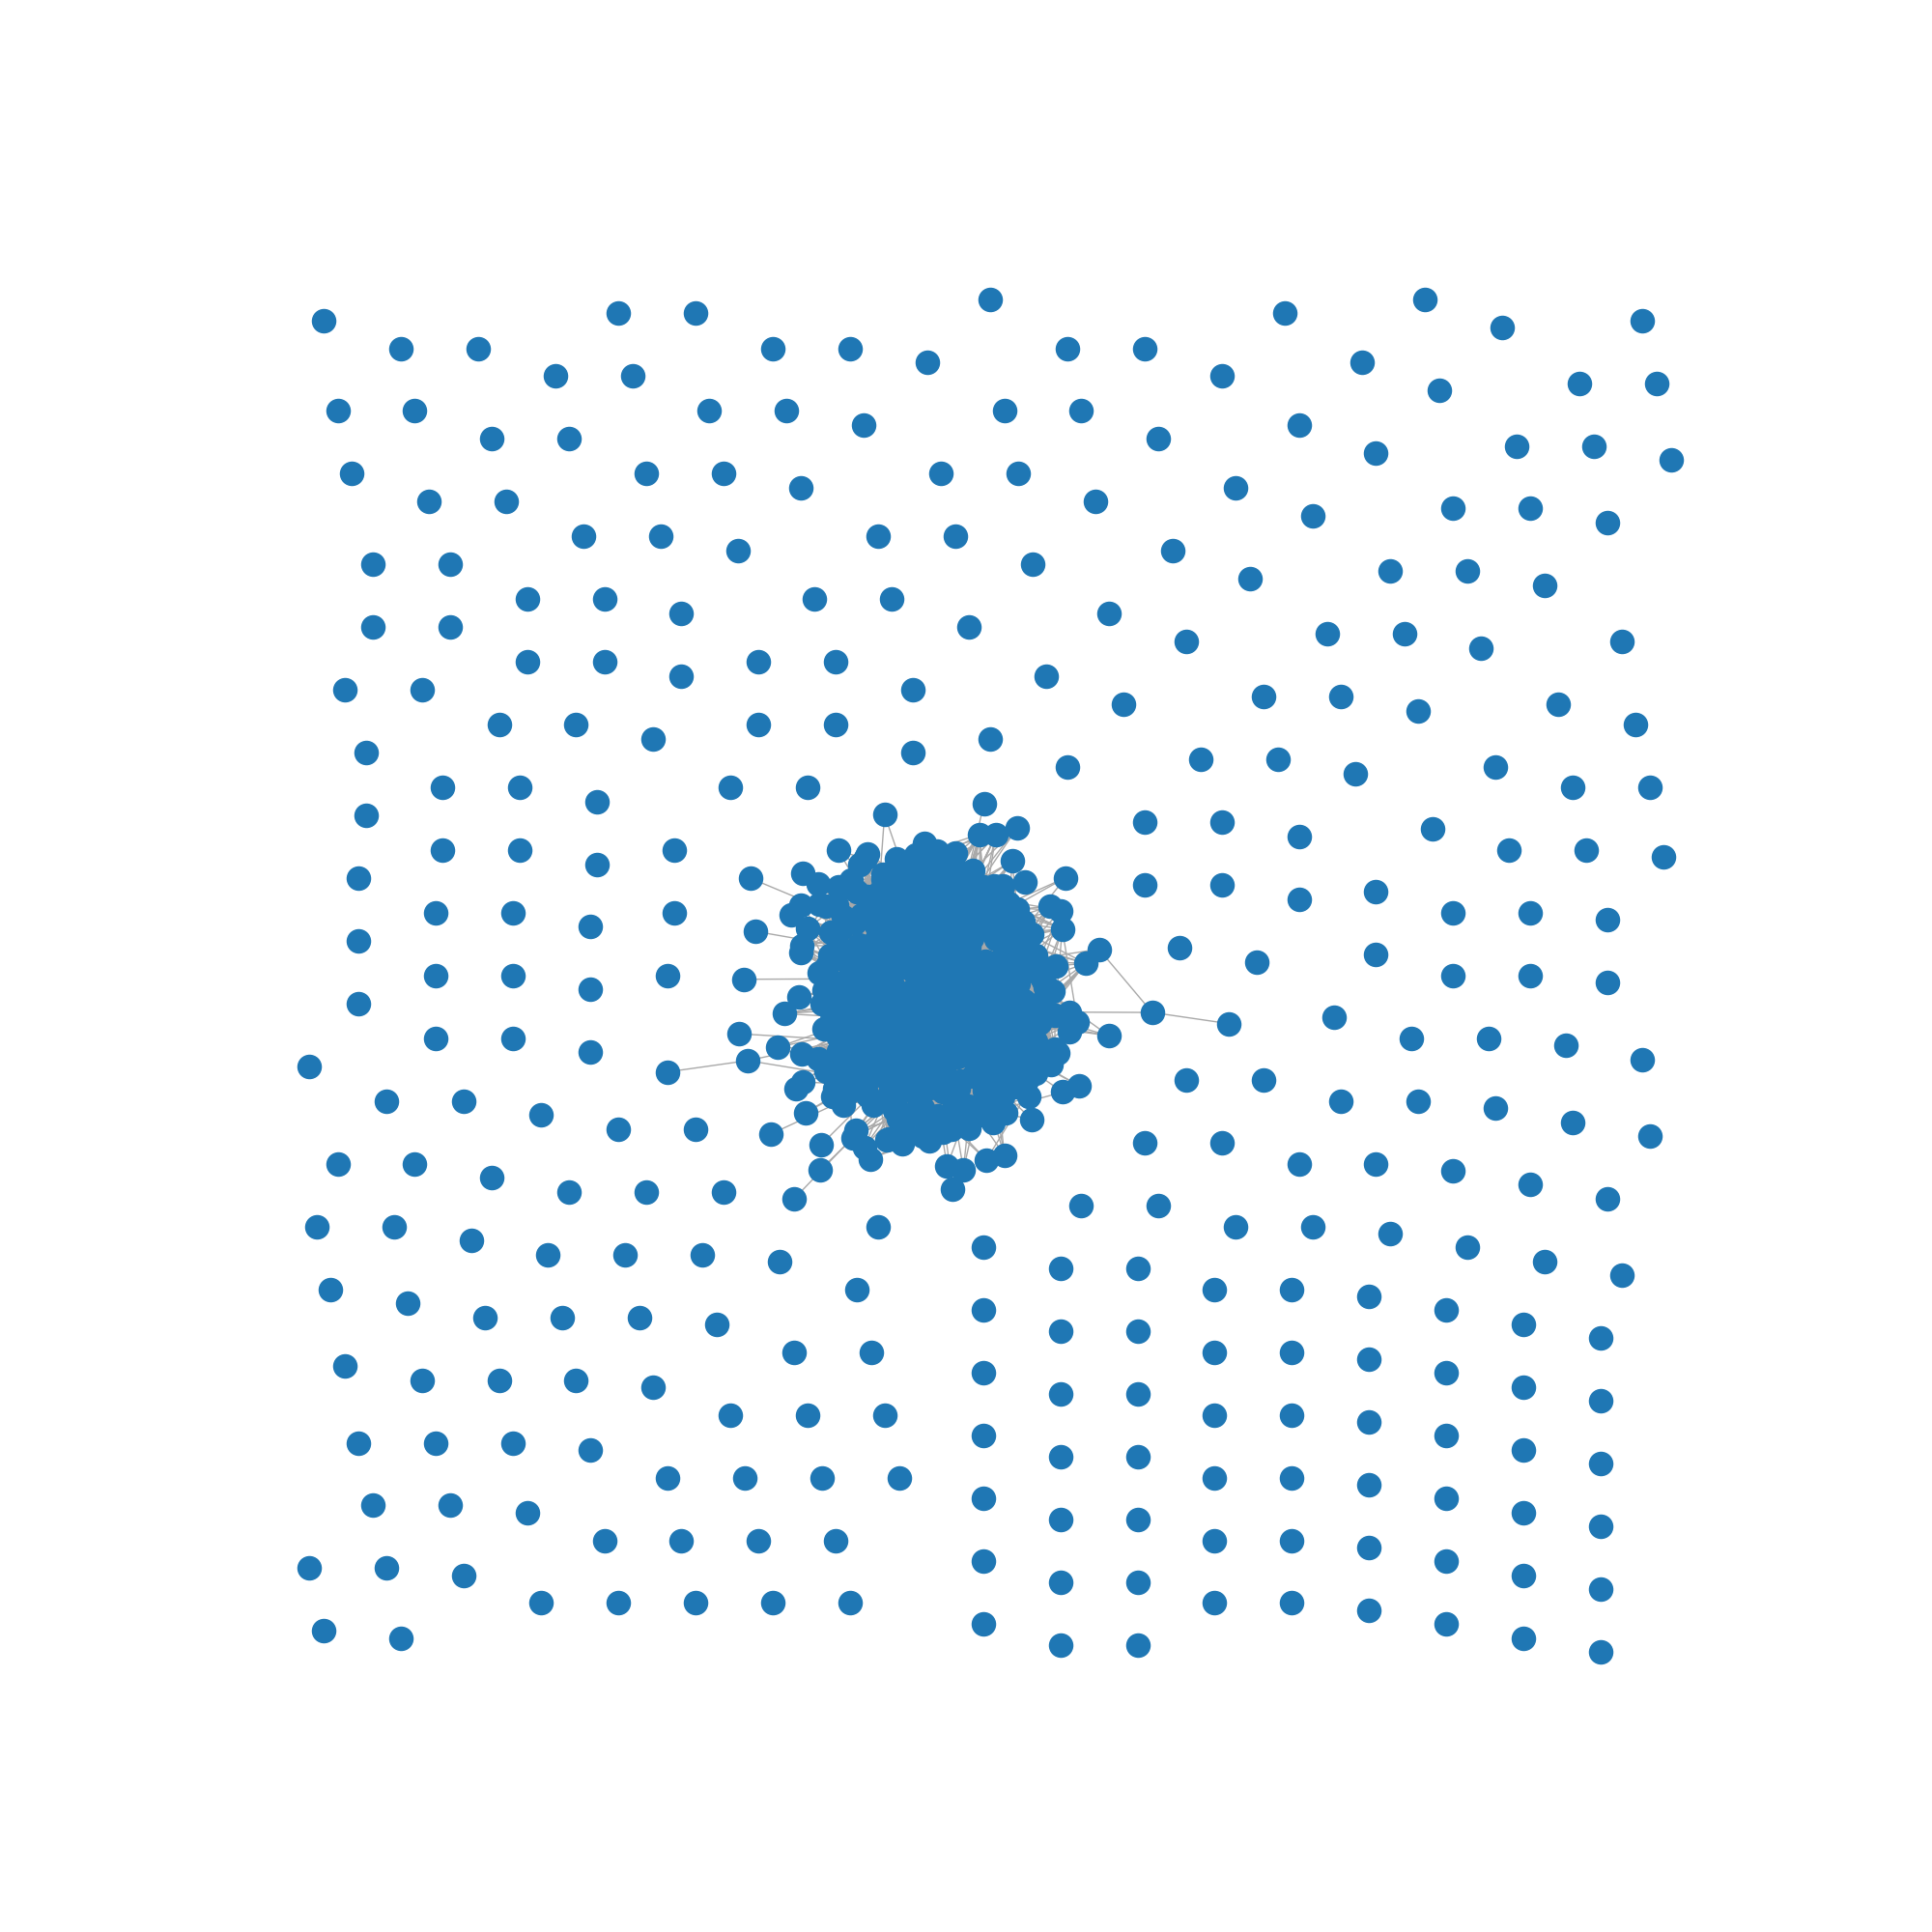
\includegraphics[width=.25\textwidth]{/files/src/.media/ego/grafo_6.png}}\hfill
    \subfloat[$u = 6$]{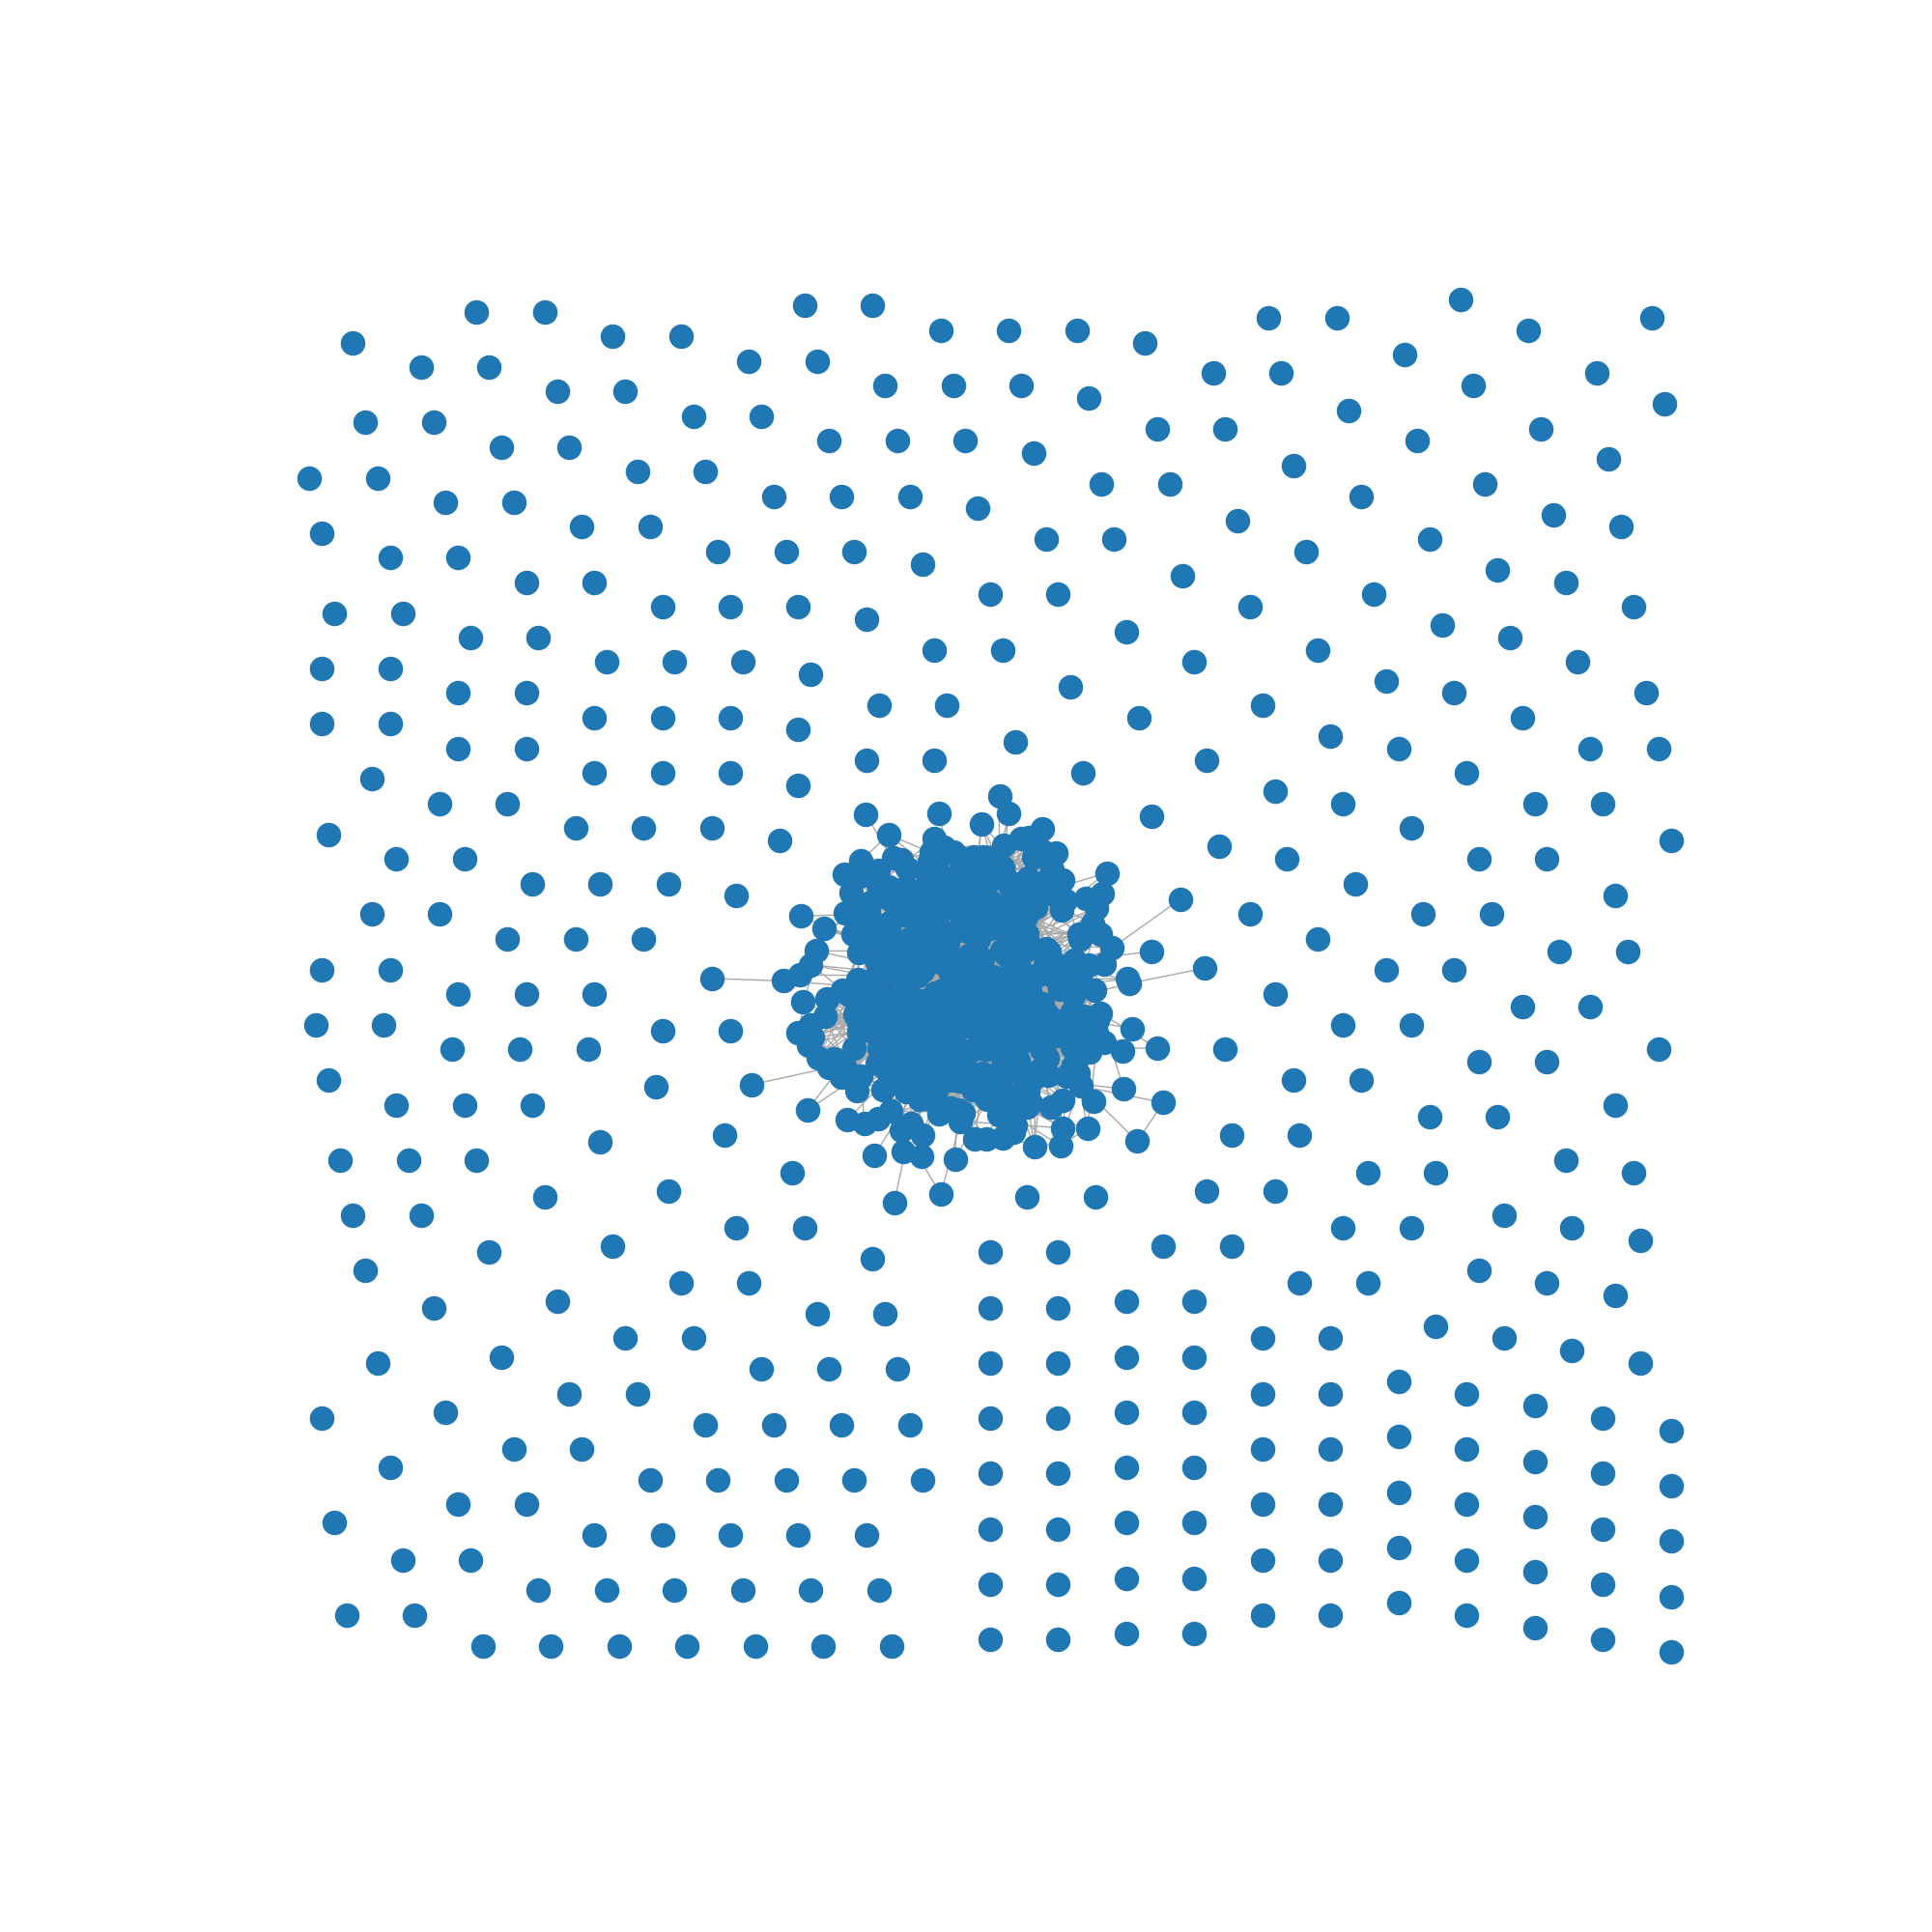
\includegraphics[width=.25\textwidth]{/files/src/.media/ego/grafo_7.png}}\hfill
    \subfloat[$u = 7$]{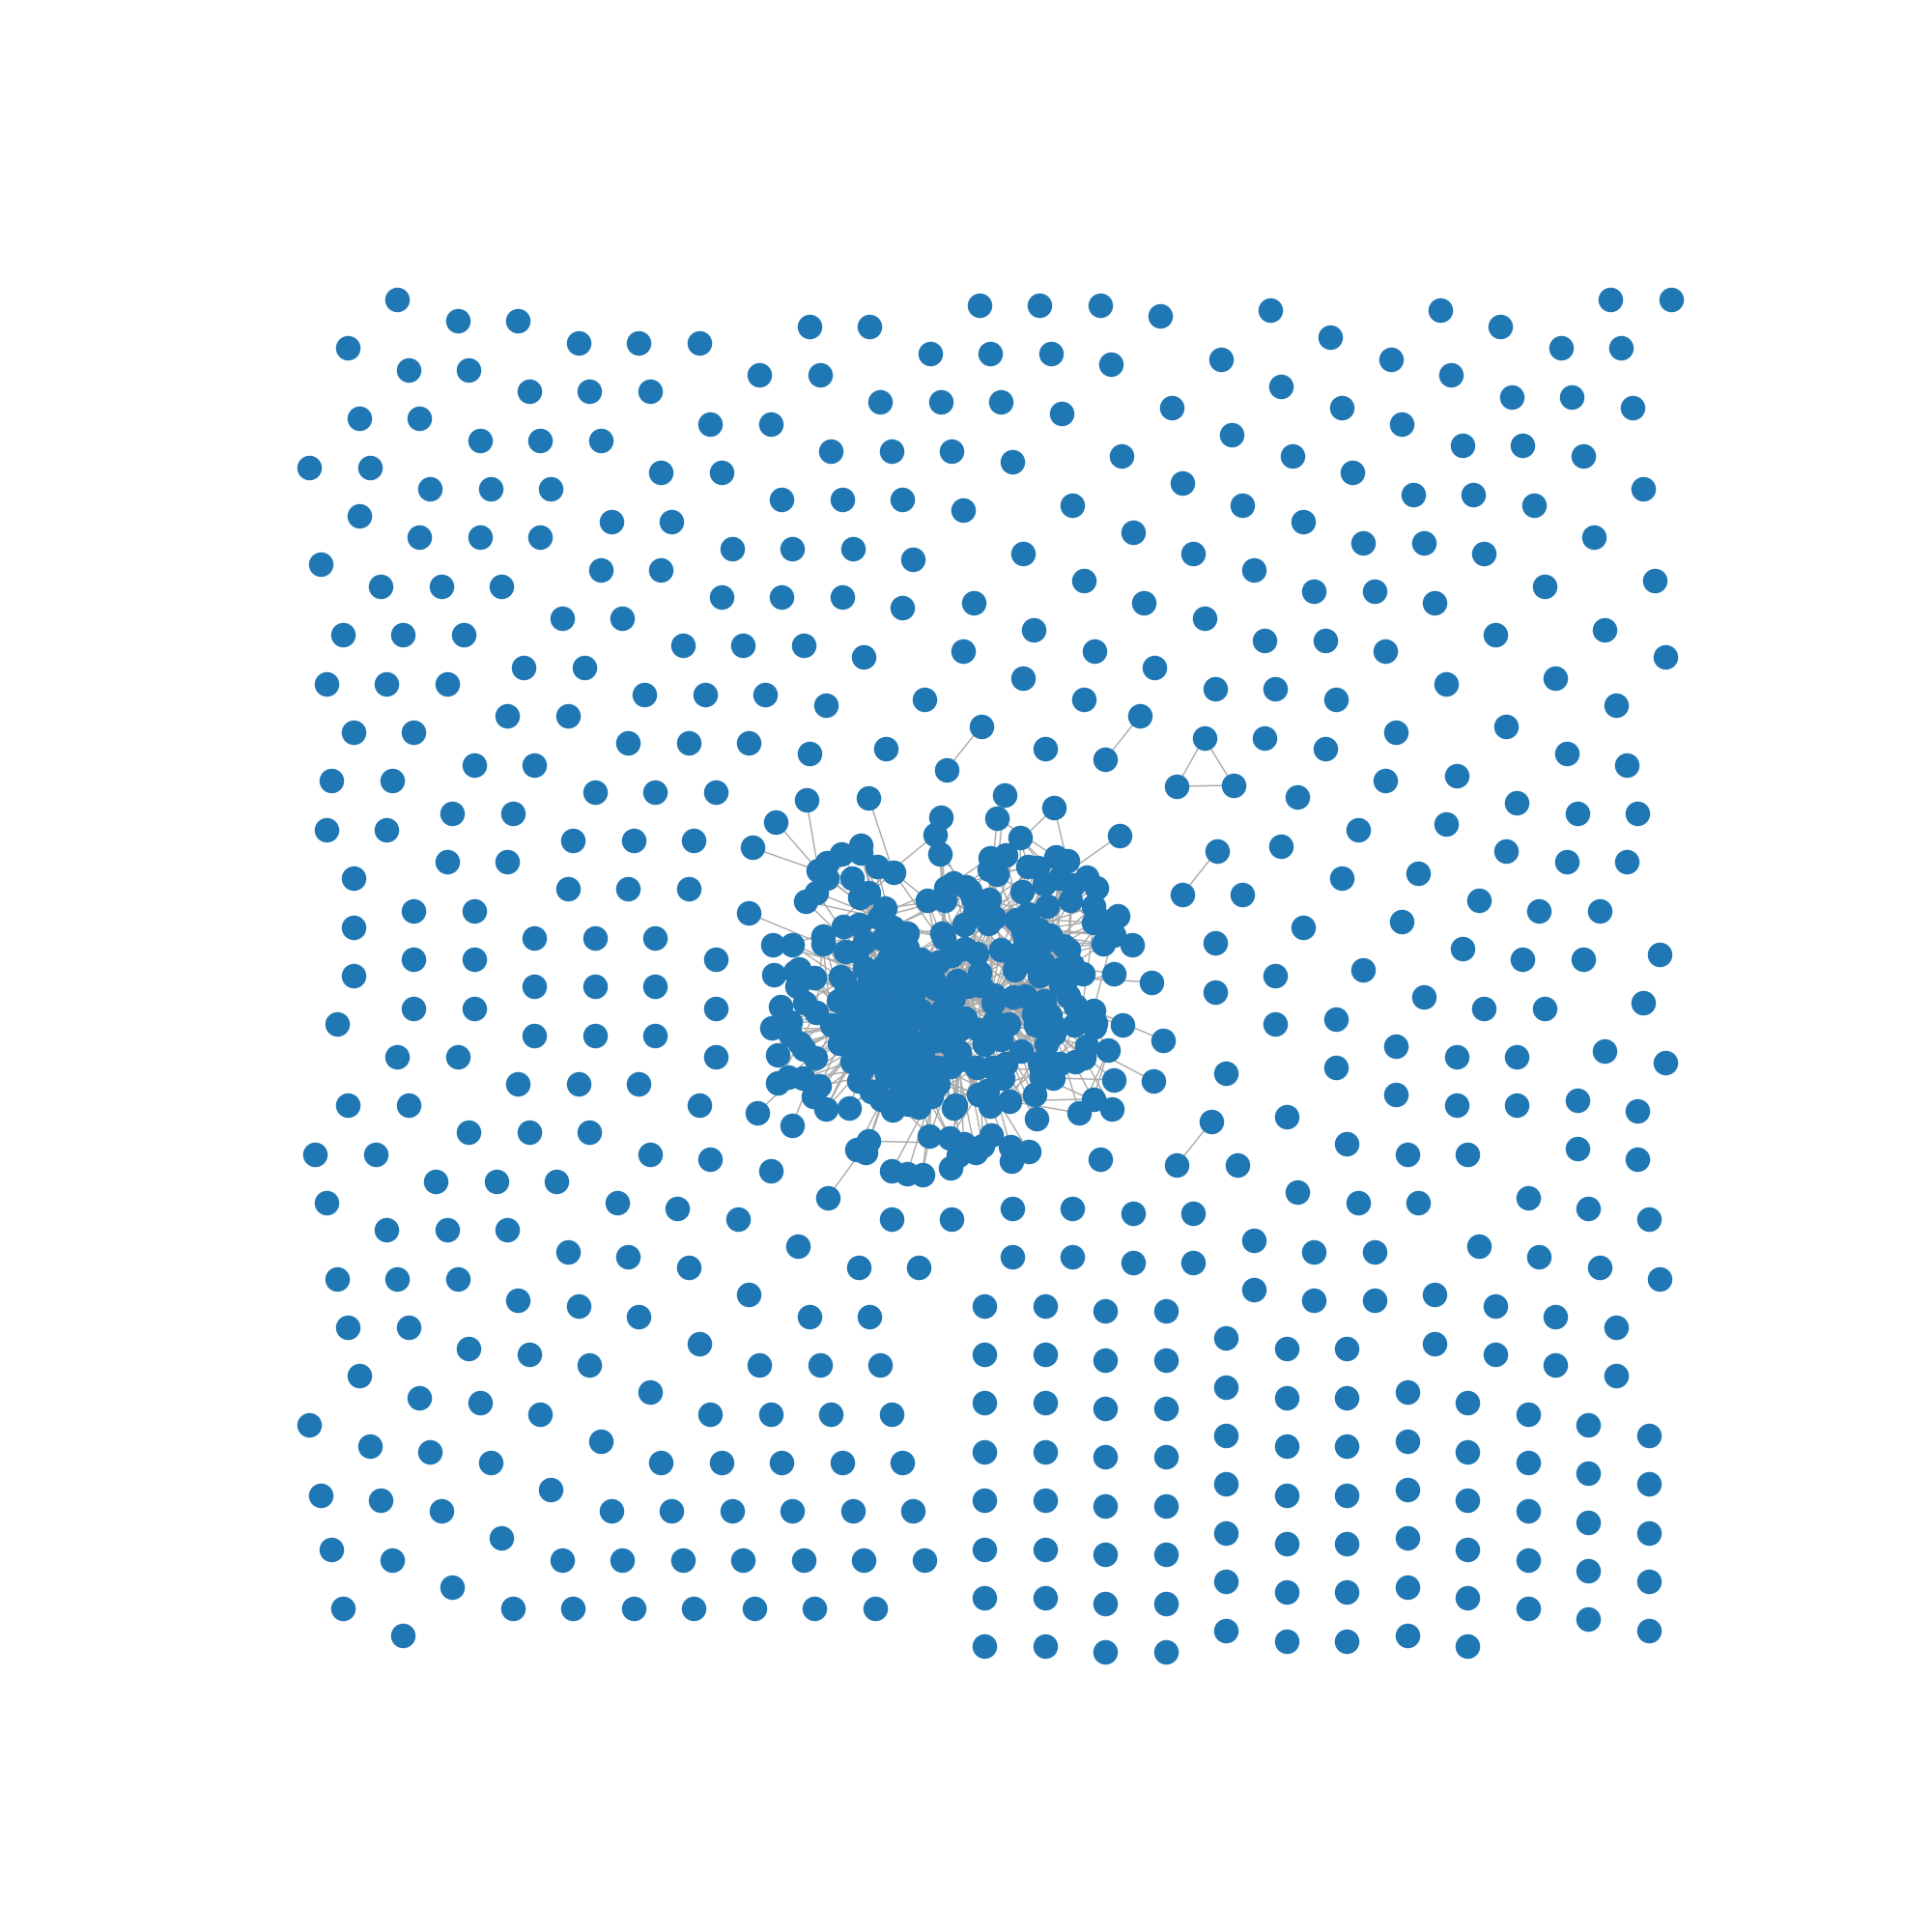
\includegraphics[width=.25\textwidth]{/files/src/.media/ego/grafo_8.png}}\hfill    
    \\[\smallskipamount]
    \subfloat[$u = 8$]{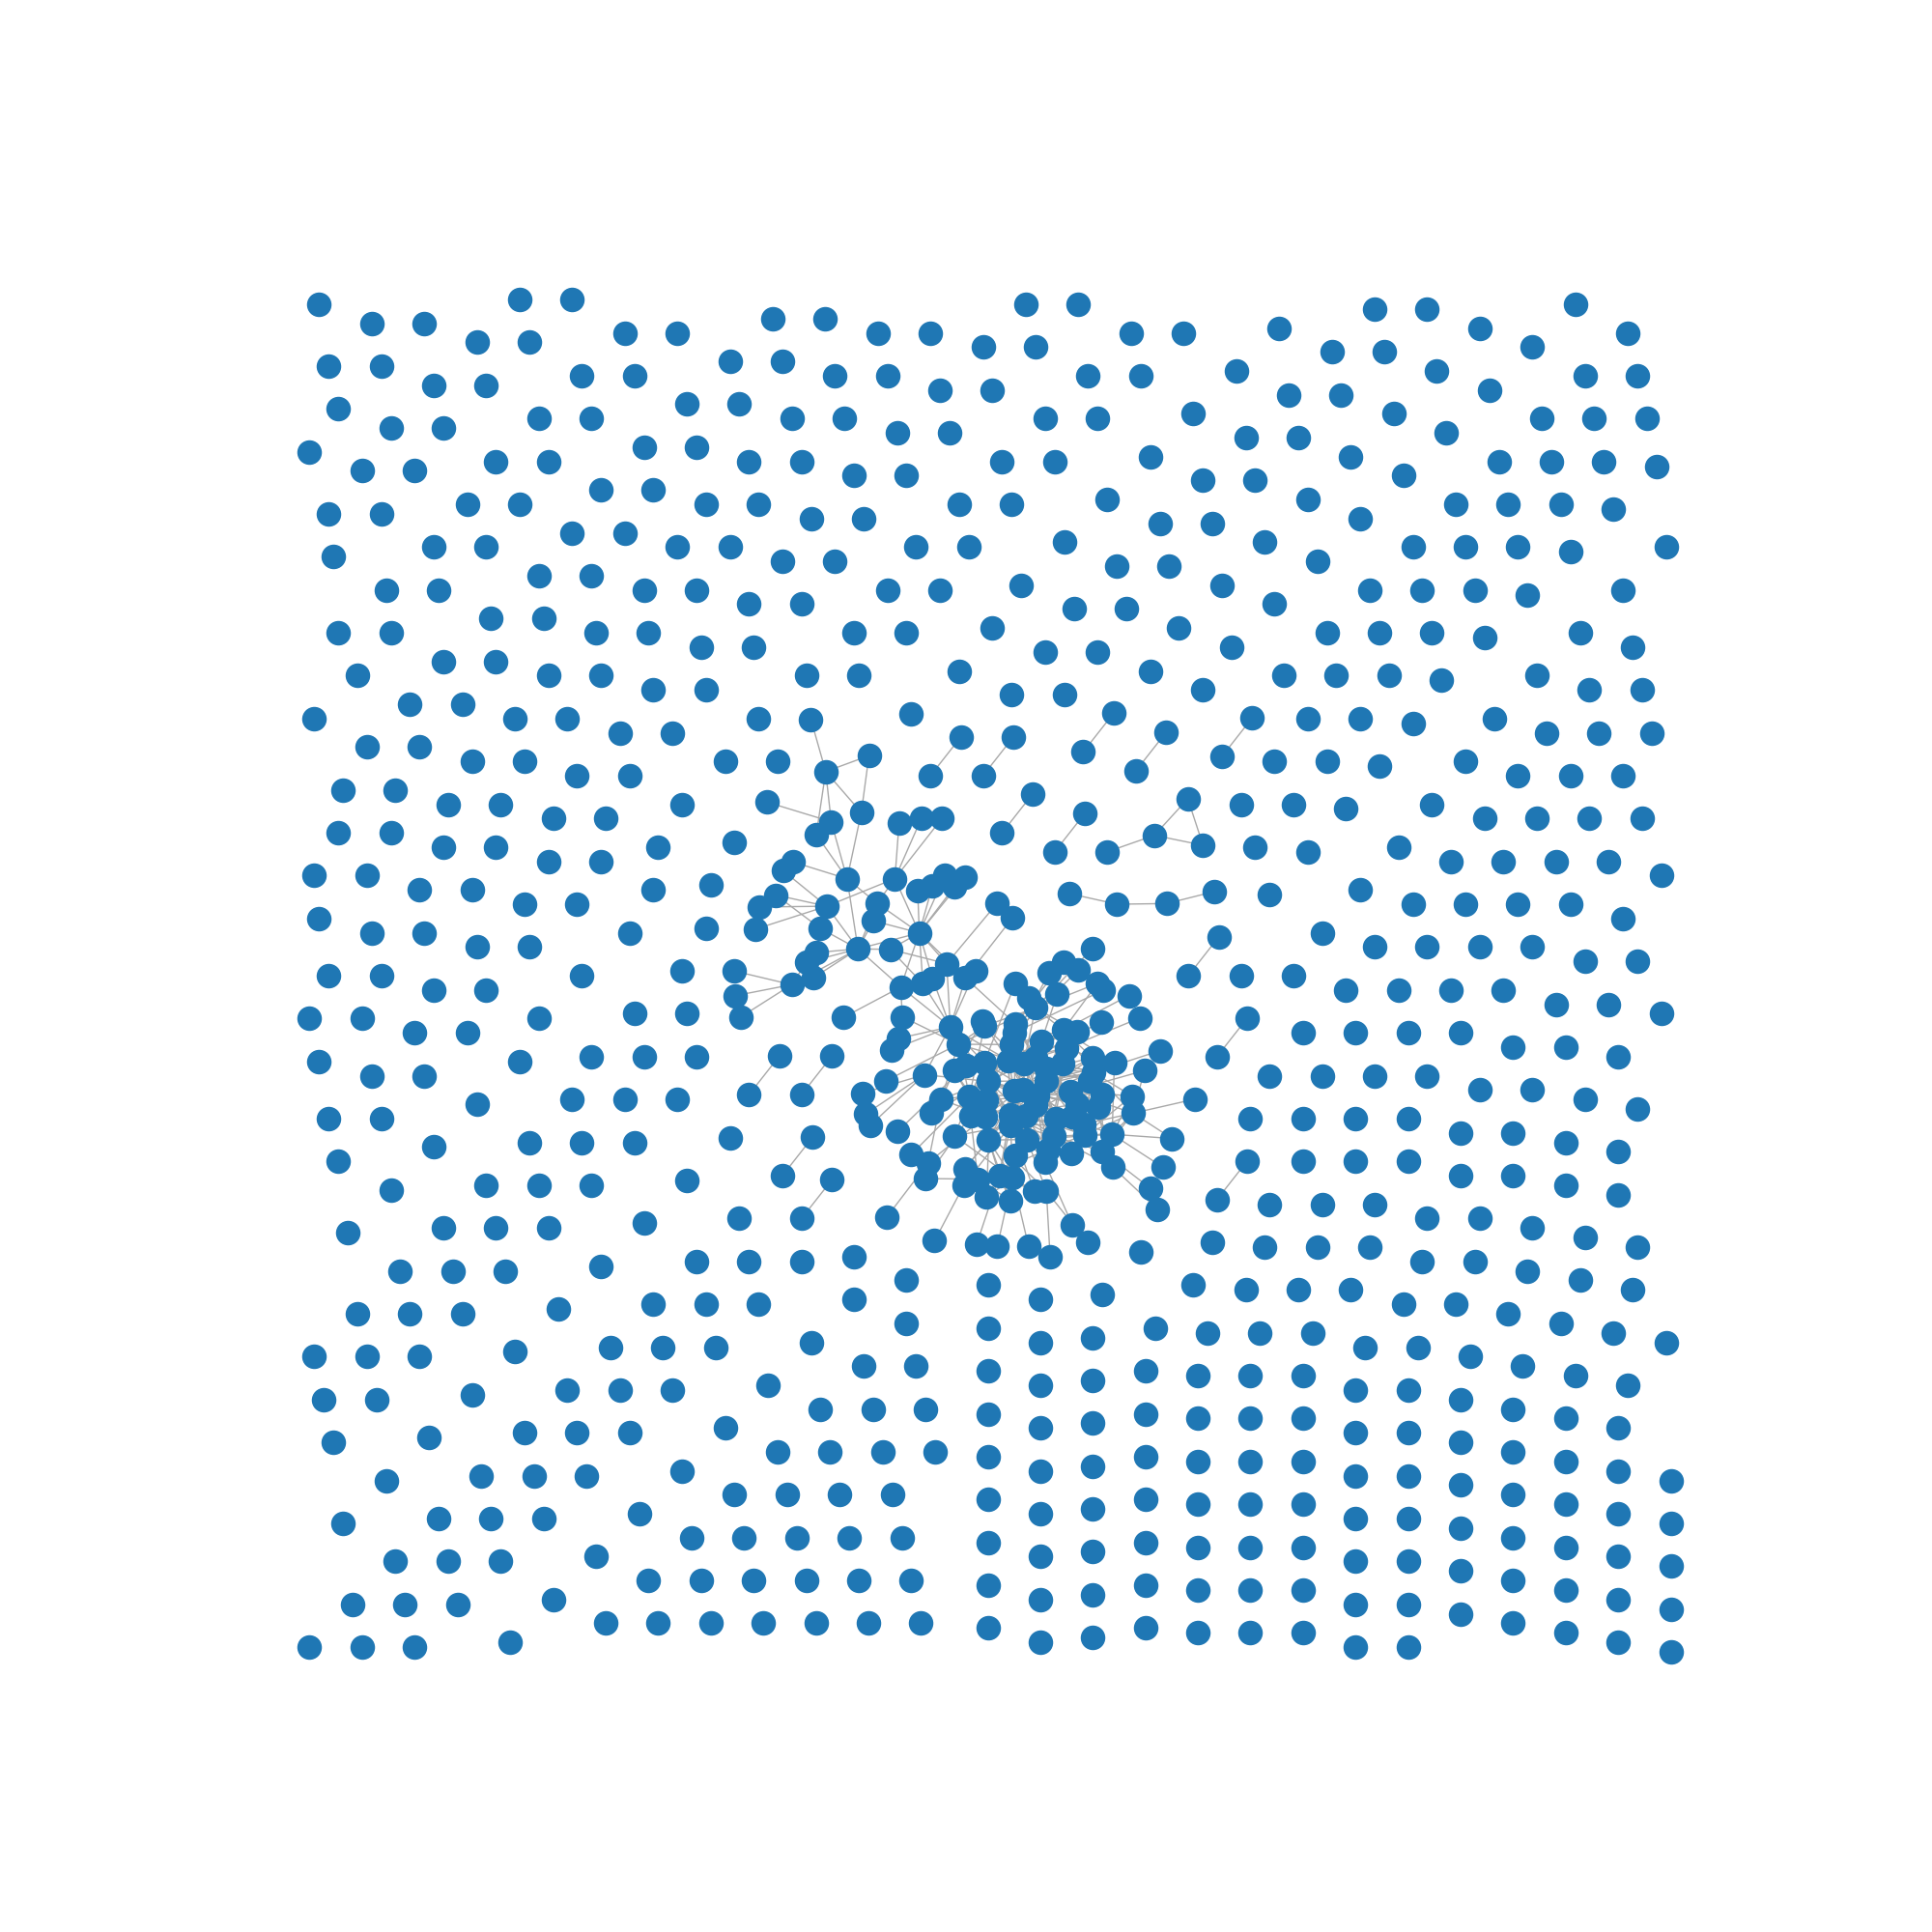
\includegraphics[width=.25\textwidth]{/files/src/.media/ego/grafo_9.png}}\hfill
    \subfloat[$u = 9$]{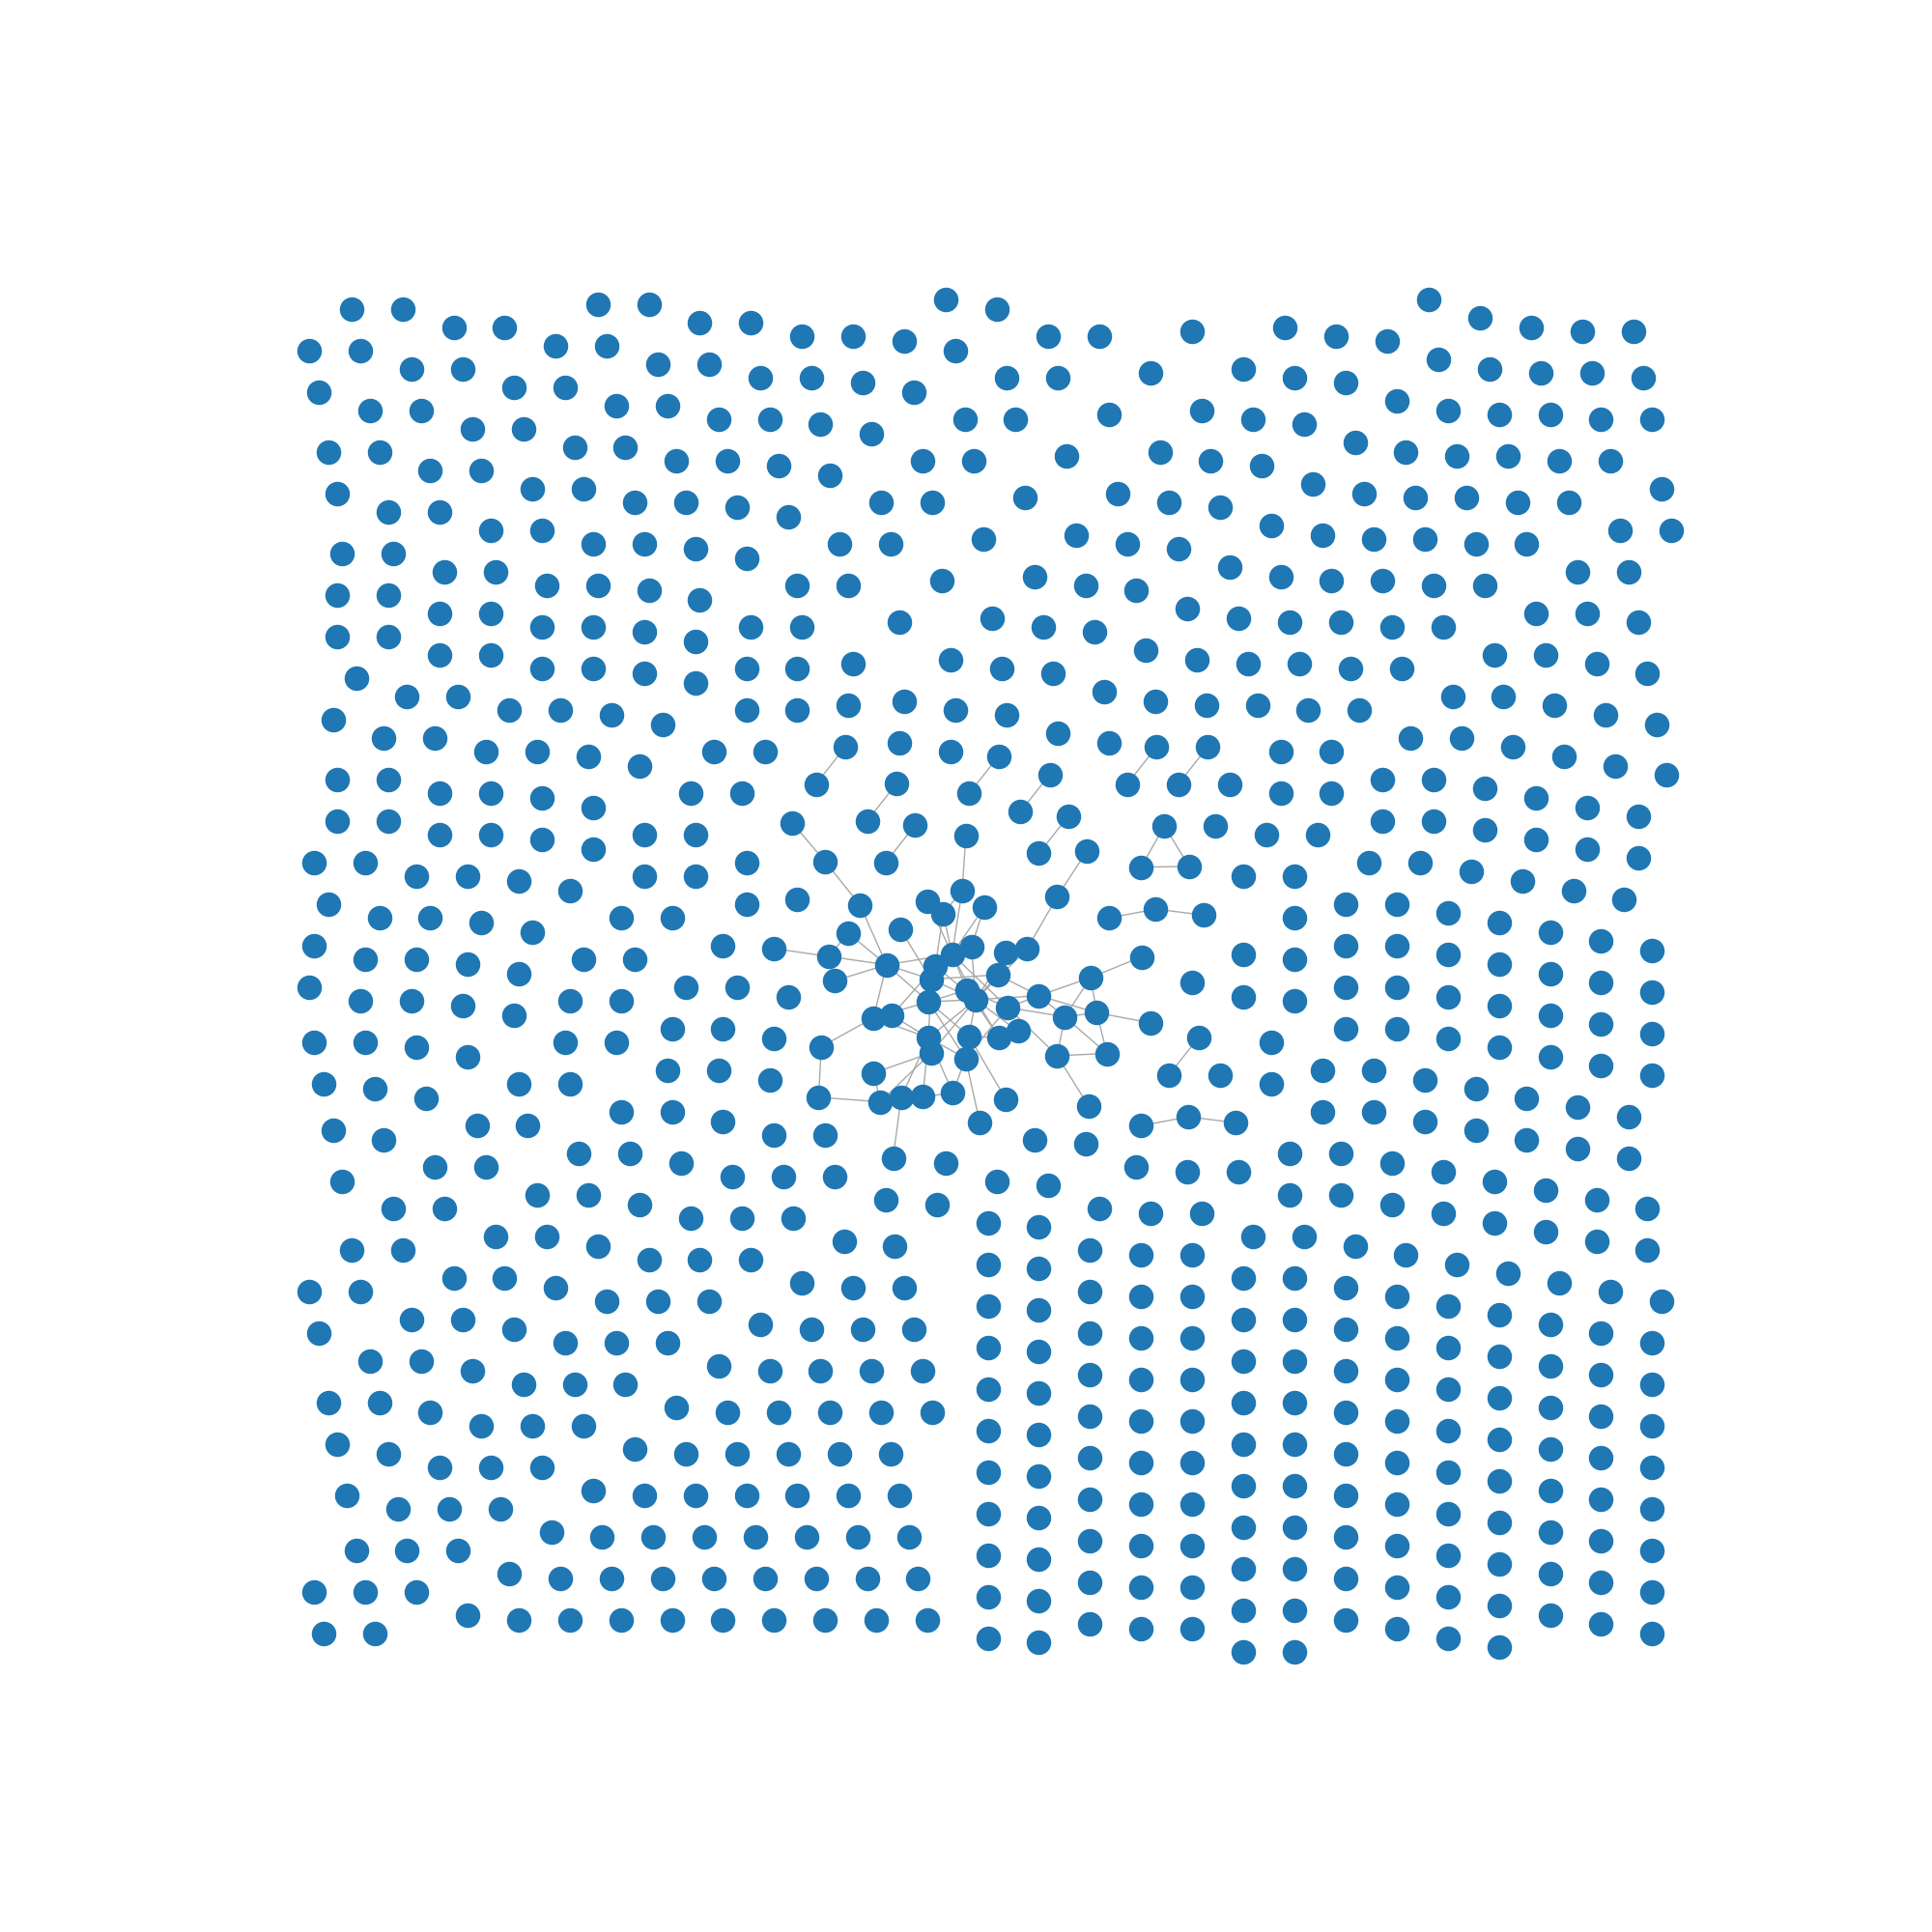
\includegraphics[width=.25\textwidth]{/files/src/.media/ego/grafo_10.png}}\hfill
    \subfloat[$u = 10$]{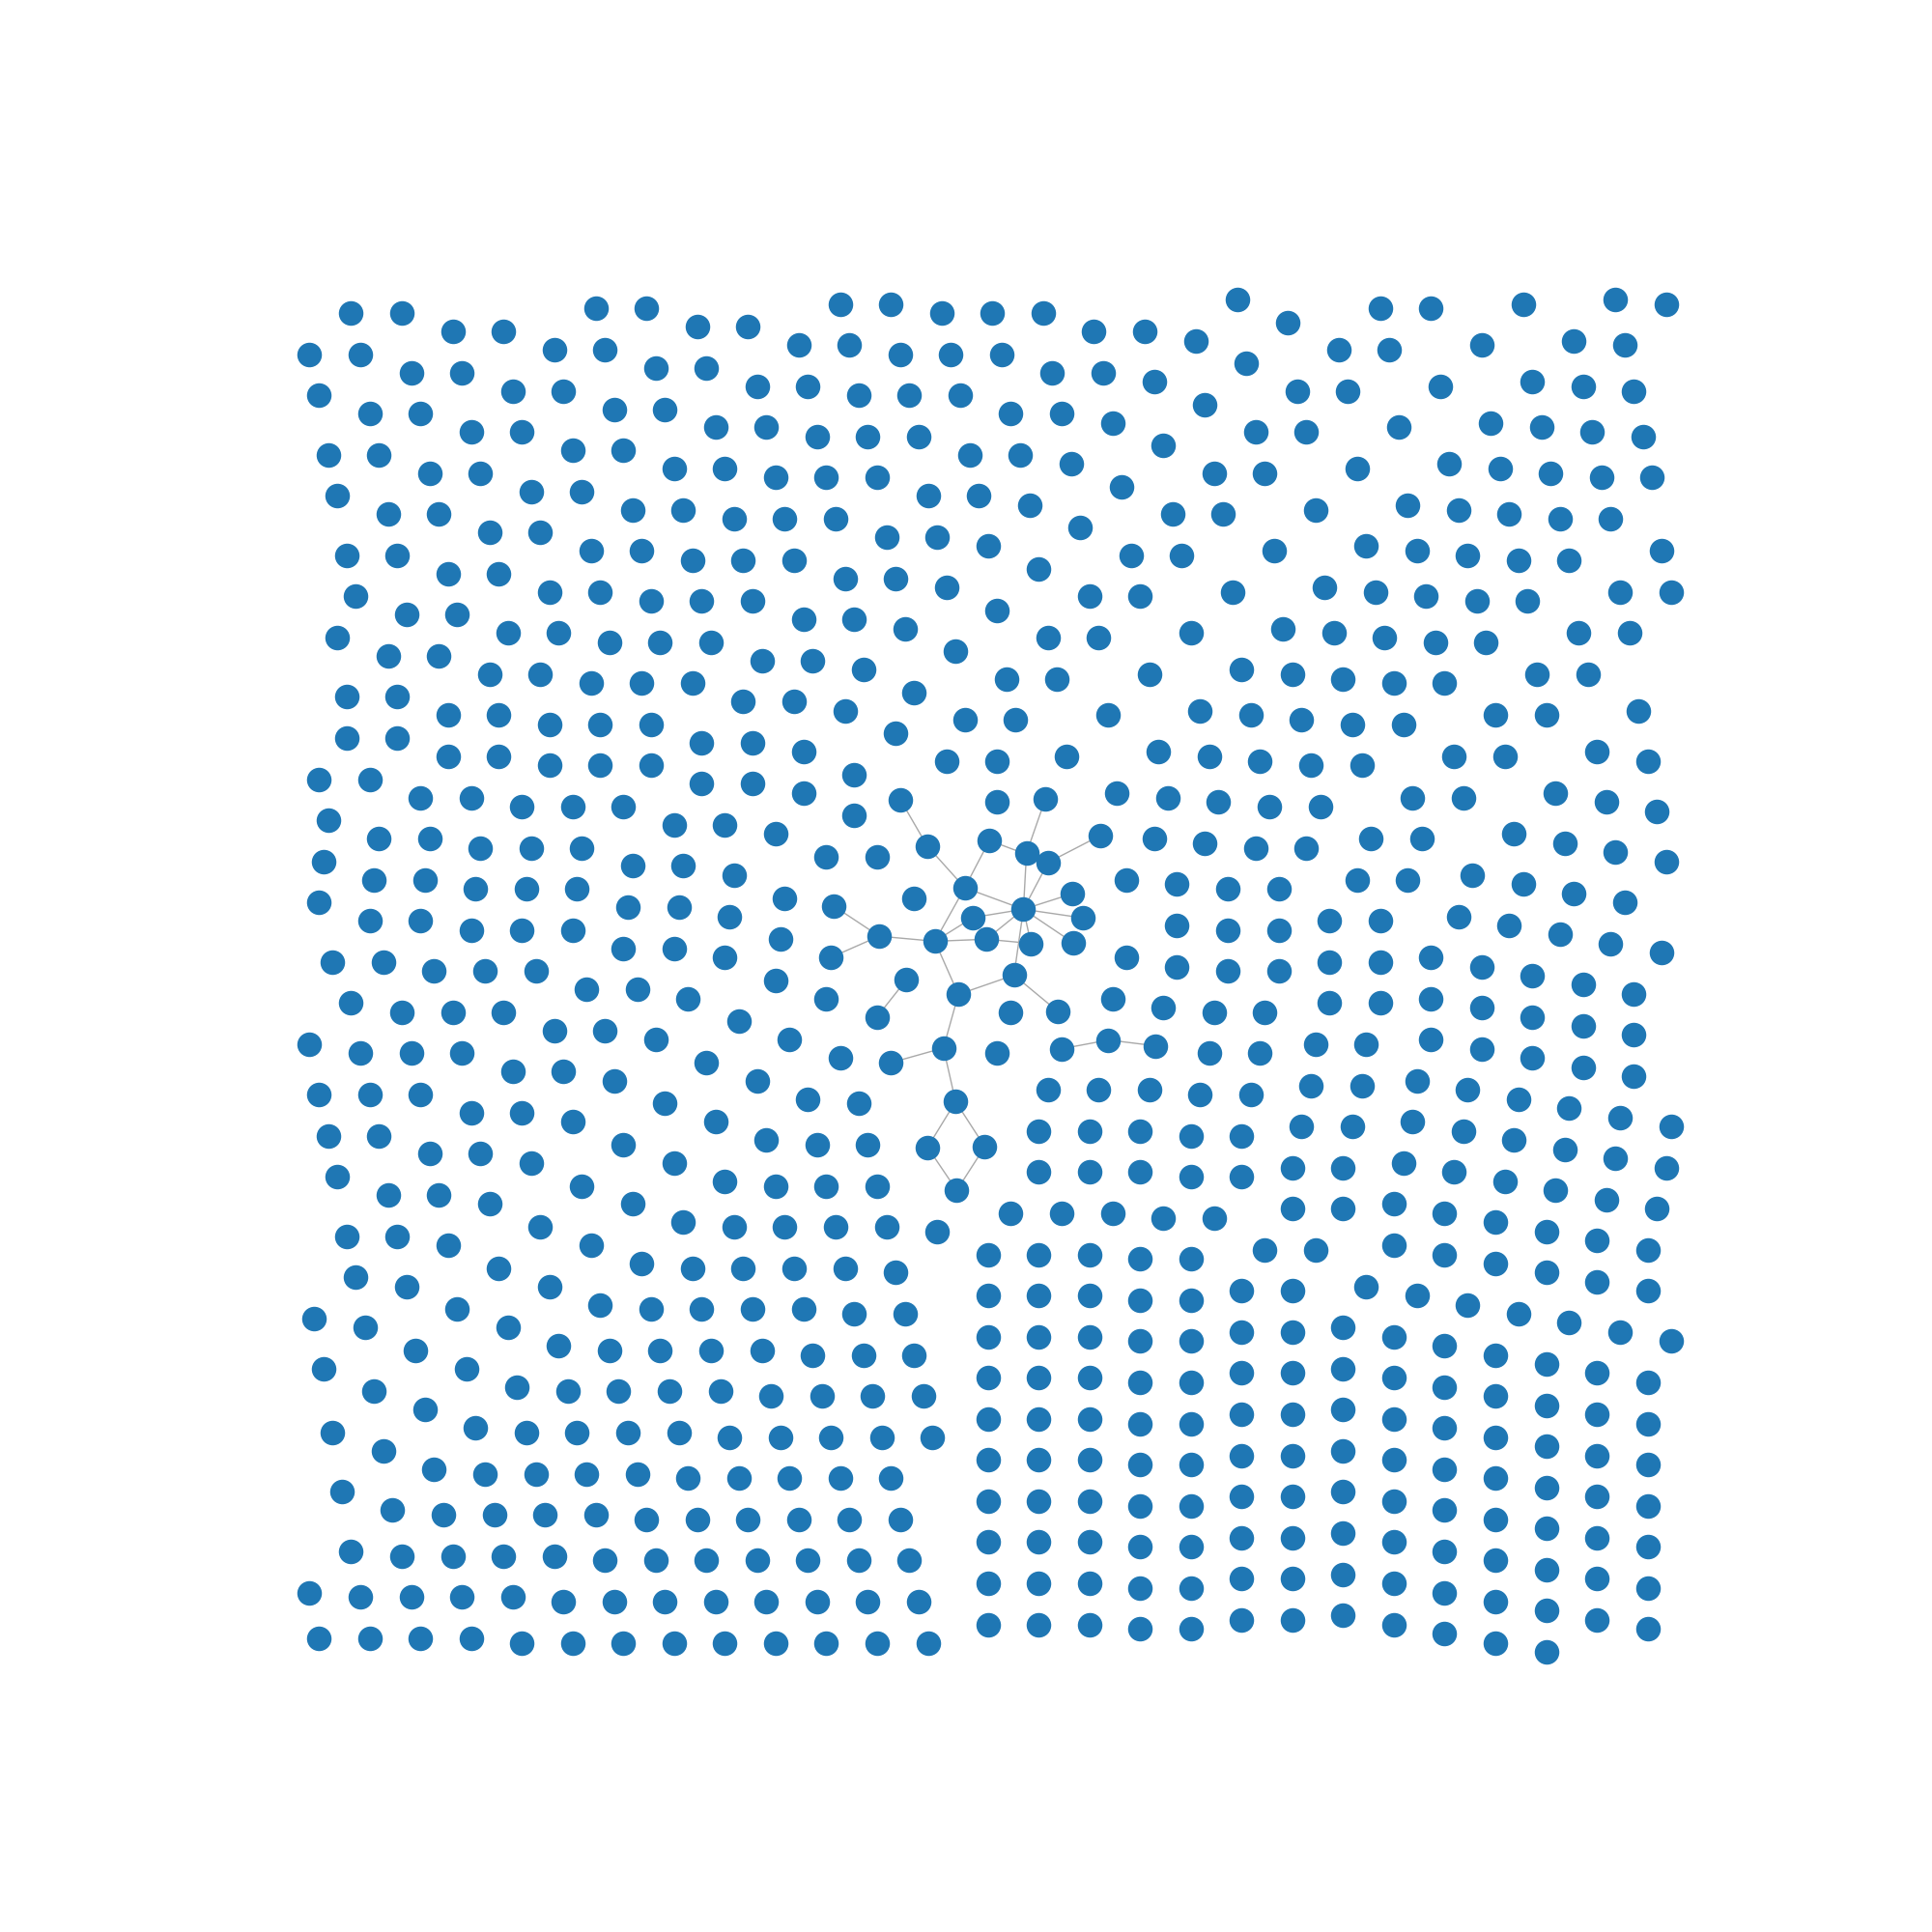
\includegraphics[width=.25\textwidth]{/files/src/.media/ego/grafo_11.png}}\hfill
    \subfloat[$u = 11$]{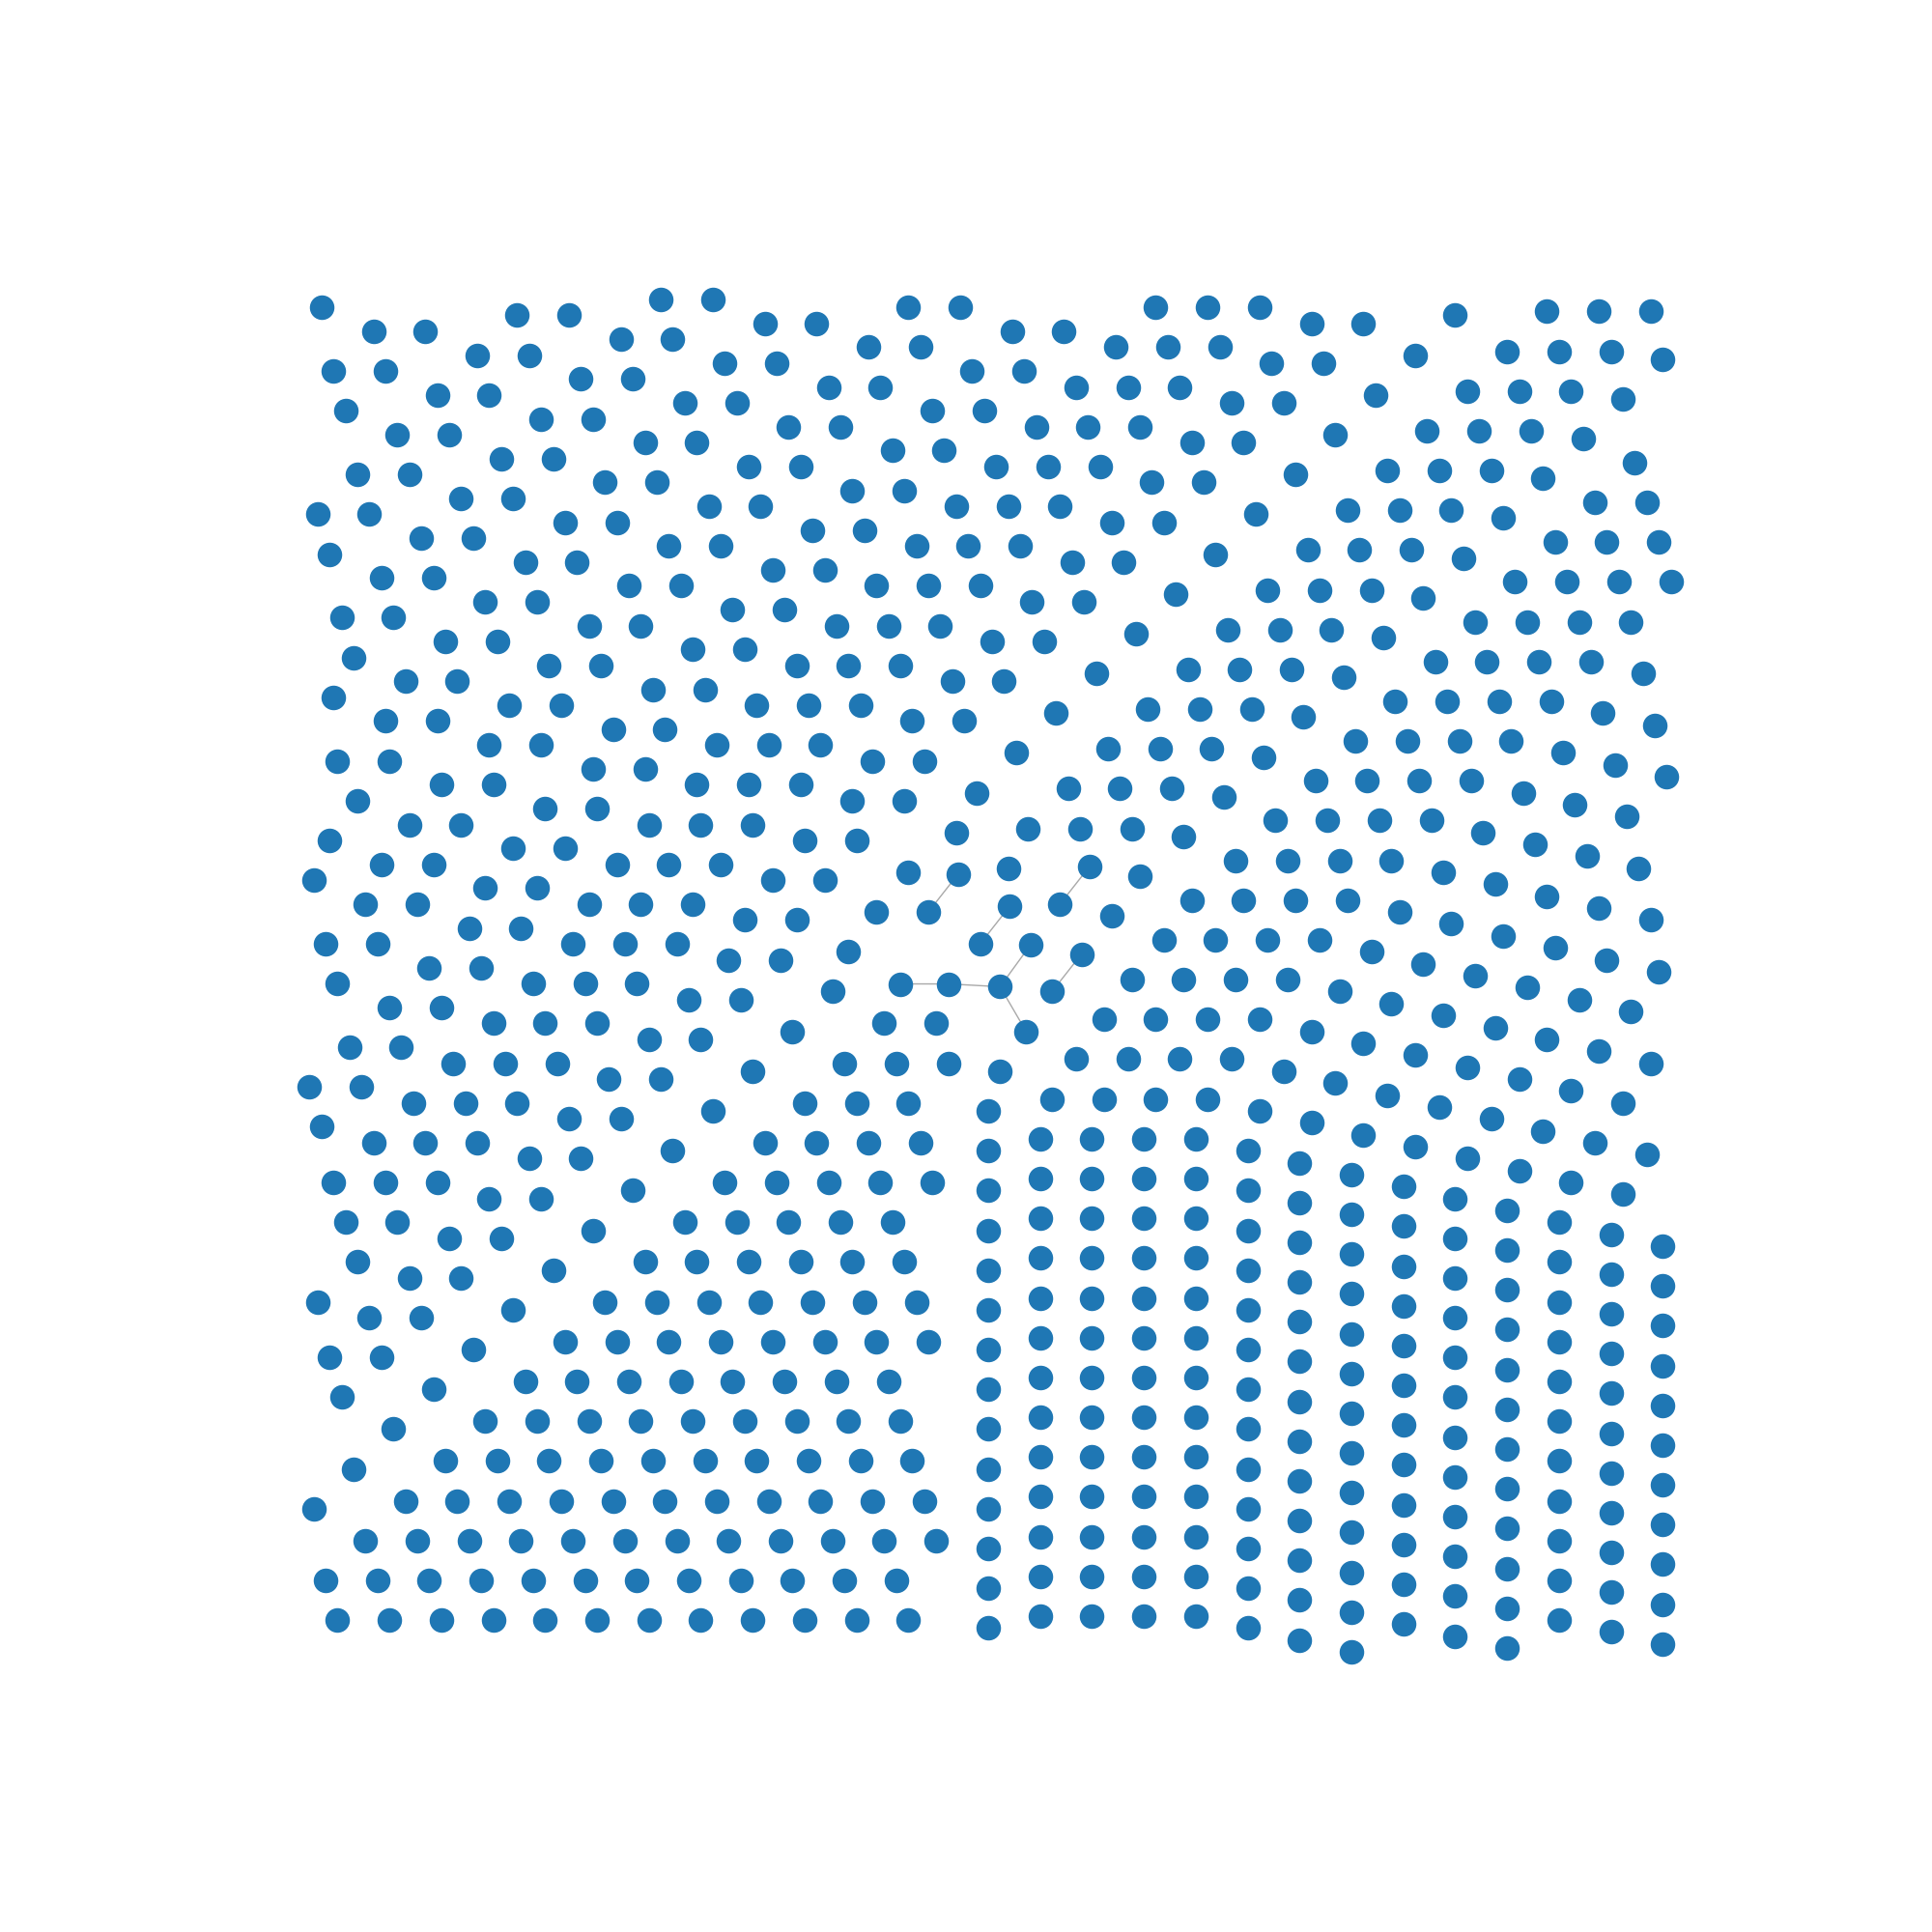
\includegraphics[width=.25\textwidth]{/files/src/.media/ego/grafo_12.png}}\hfill
    \\[\smallskipamount]
    \subfloat[$u = 12$]{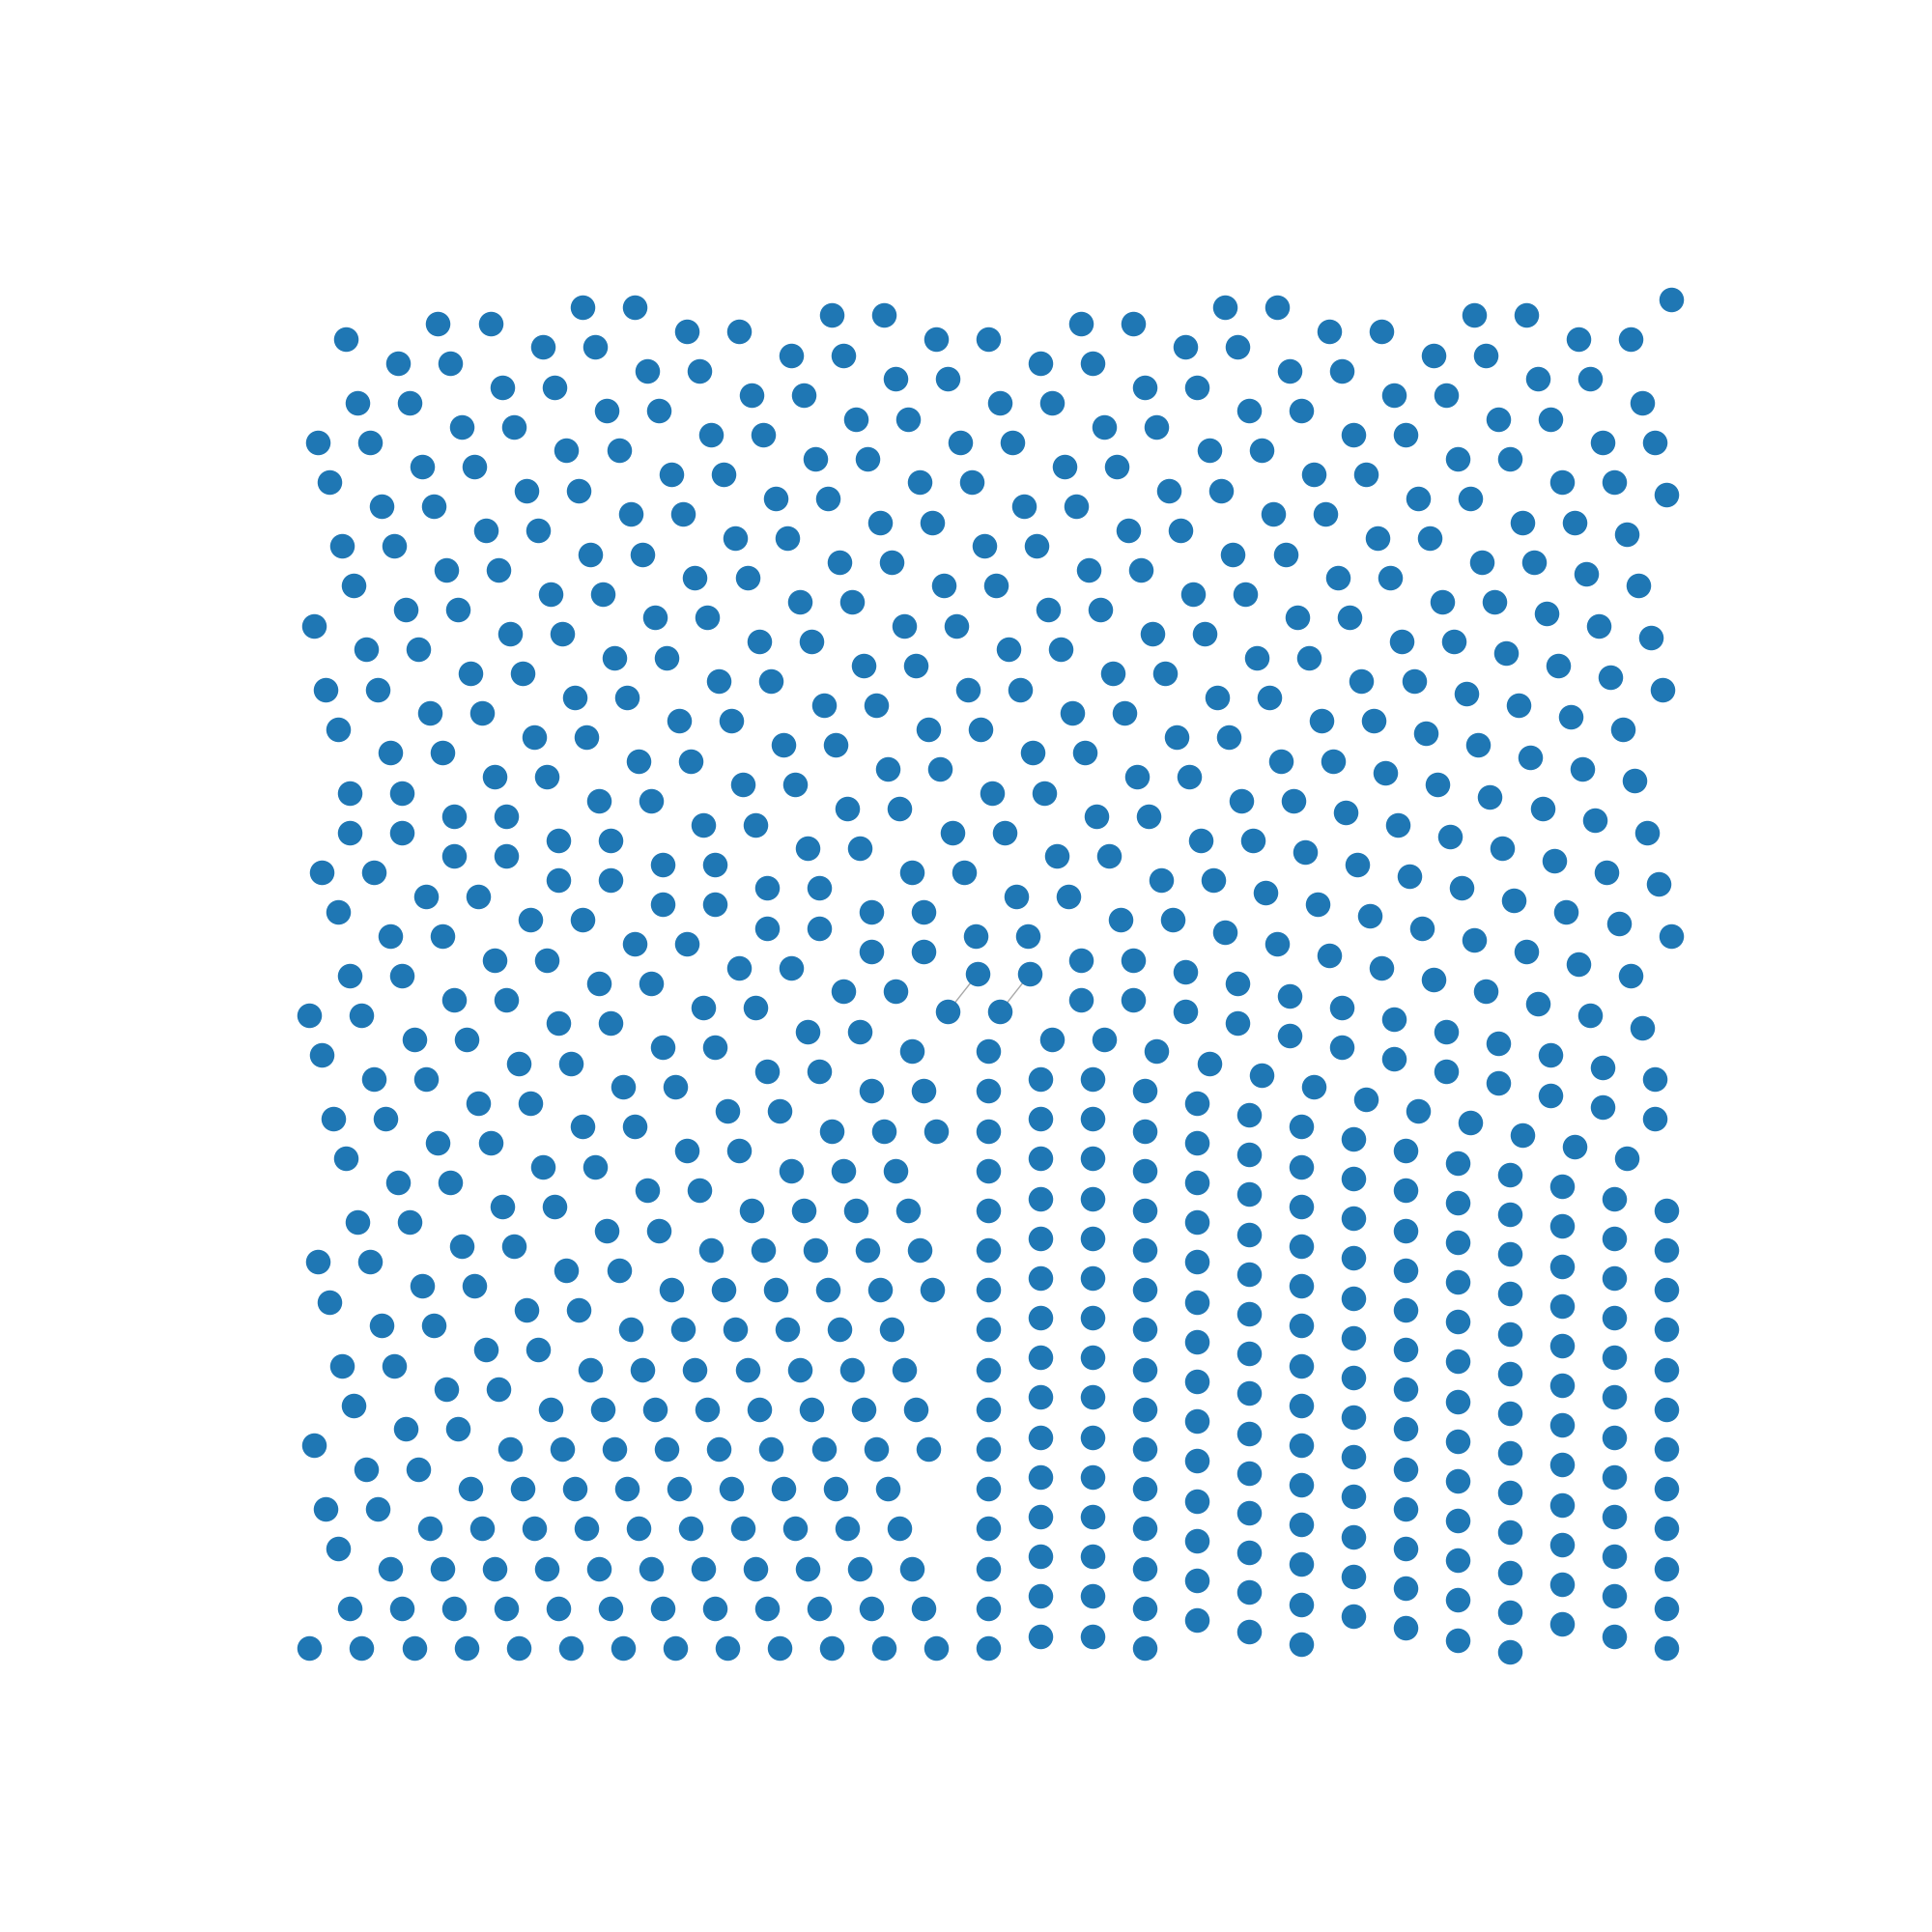
\includegraphics[width=.25\textwidth]{/files/src/.media/ego/grafo_13.png}}
    \\[\smallskipamount]
    \caption{Todos los grafos correspondientes a los diferentes umbrales, tomados a partir de las matrices de conectividad $\mathbf{C}\ \mathbf{C}^t > u$. Los números debajo de cada imagen indican el umbral utilizado.} \label{grafos_aproximados}
    %indican la cantidad de conexiones
\end{figure}




% === COMPARACION === %

\vspace{2em}
\subsection{Comparación con la red original}

% aca creo que quedaria mejor primero mencionar todos los metodos
% despues mostrar tabla resultados
% y grafico
% y despues hacer el analisis
% ej:

Nos encontramos con diferentes grafos construidos en base a los atributos en \textbf{C}. Buscamos ahora comparar nuestras aproximaciones con la red original. 

\vspace{1em}
Un primer acercamiento a este problema puede ser calcular la cantidad de \textit{posiciones coincidentes} entre las matrices de adyacencia y dividir por los elementos totales. La lógica por detrás del método es que nuestros grafos serán más similares entre sí por cada conexión y `no conexión' acertada. %Entonces, por cada 0 y 1 coincidente en nuestra aproximación y \textbf{E} nos acercaríamos más a un 100\% de similitud. 

%\vspace{1em}
Otros dos métodos de comparación posibles son la comparación de matrices por \textit{adyacencia estirada} ---donde se computa la correlación entre los vectores estirados de las matrices---, y la comparación por \textit{listas de autovalores} ---donde se computa la correlación entre los vectores ordenados de autovalores---. La correlación, por su parte, es una covarianza normalizada con valores en (-1, 1), donde números mayores indican una mayor similitud. Se describe por la siguiente fórmula:

\vspace{1em}
\begin{equation}
    Corr(x, y) = \frac{(x - \mu_{x}) \cdot (y - \mu_{y})}{\sqrt[]{(x - \mu_{x})^{2} \cdot (y - \mu_{y})^{2}}}
    \label{eq:corr}
\end{equation}

\vspace{1em}
\noindent siendo $\mu$ el valor medio de los vectores.

\vspace{1em}
\begin{figure}[!htbp]
    \begin{tabular}{ |c|c|c|c|c| } 
    \hline
    aproximación & conexiones & coincidentes & adyacencia estirada & autovalores \\
    \hline
    0            &298,799                 & 7.61\%\     & 1.25\%\               & 47.99\%\ \\
    1            &213,902                 & 32.95\%\    & 2.32\%\               & 60.86\%\ \\
    2            &127,382                 & 58.57\%\    & 2.94\%\               & 62.98\%\ \\
    3            &86,847                  & 70.99\%\    & 5.86\%\               & 75.48\%\ \\
    4            &43,091                  & 84.16\%\    & 9.61\%\               & 88.29\%\ \\
    5            &16,850                  & 91.54\%\    & 10.96\%\              & 94.28\%\ \\
    6            &5,727                   & 94.32\%\    & 9.75\%\               & 95.06\%\ \\
    7            &1,517                   & 95.21\%\    & 6.90\%\               & 92.64\%\ \\
    8            &405                     & 95.40\%\    & 4.15\%\               & 85.62\%\ \\
    9            &108                     & 95.45\%\    & 2.34\%\               & 77.52\%\ \\
    10           &36                      & 95.46\%\    & 1.35\%\               & 63.31\%\ \\
    11           &8                       & 95.46\%\    & 0.50\%\               & 55.00\%\ \\
    12           &2                       & 95.46\%\    & 0.055\%\              & 46.19\%\ \\
    13           &0                       & 95.46\%\    & 0.0\%\                & 0.0\%\  \\
    \hline
    \end{tabular} \\
    \bigskip
    \caption{Similitud elemento a elemento de las matrices de adyacencia, la primer columna representa el umbral tomado para la aproximación y la segunda la cantidad de aristas del grafo (la red `ego' original cuenta con 14.024). Las columnas siguientes miden el porcentaje de similitud respecto a \textbf{E} en función de cada método propuesto.} \label{promedio_similaridad}
\end{figure}

\vspace{1em}
\noindent \textsc{Resultados}. Como se puede observar en la figura (\ref{promedio_similaridad}.), los grafos con muy pocas conexiones (por ejemplo, para $u > 10$), tienen los valores más altos de similitud por \textit{posiciones coincidentes}, mientras que otros con cantidad de aristas similares a la red original ---como $u = 5$ o $u = 6$, que cuentan con 16,850 y 5,727 conexiones respectivamente---, parecerían ser peores aproximaciones. Esto se da por la naturaleza rala de nuestras matrices de adyacencia. La de la red `ego' \textbf{E} es de $786 \times 786$, con 617,796 elementos, y tan solo 28,048 (4.54\%) no nulos. Es decir, es rala en un 95.46\%. Es por esto que comparar elemento a elemento no prueba ser un método muy descriptivo de qué tan buena es una aproximación, ya que cualquiera con pocos elementos coincidirá en un $\sim$ 95\%.

\vspace{1em}
En la figura (\ref{grafo_correlaciones}.) se puede apreciar que se obtienen resultados considerablemente diferentes a los de nuestro primer método de comparación si se emplean los otros. En un primer lugar, siguiéndonos de la correlación entre los vectores de \textit{adyacencia estirada}, parecería que las mejores aproximaciones son las que tienen una cantidad de aristas similar a la red original ---con los umbrales $u \in [4,7]$, ver (\ref{grafos_aproximados}.)---, mientras que los grafos vacíos con umbrales más altos pasan a tener correlación nula. De la misma forma, las \textit{listas de autovalores} muestran resultados similares, donde la mayor correlación se halla con los umbrales de valores medios y decae al avanzar hacia los extremos.  


%\vspace{1em}
\begin{figure}[!htbp]
\centering
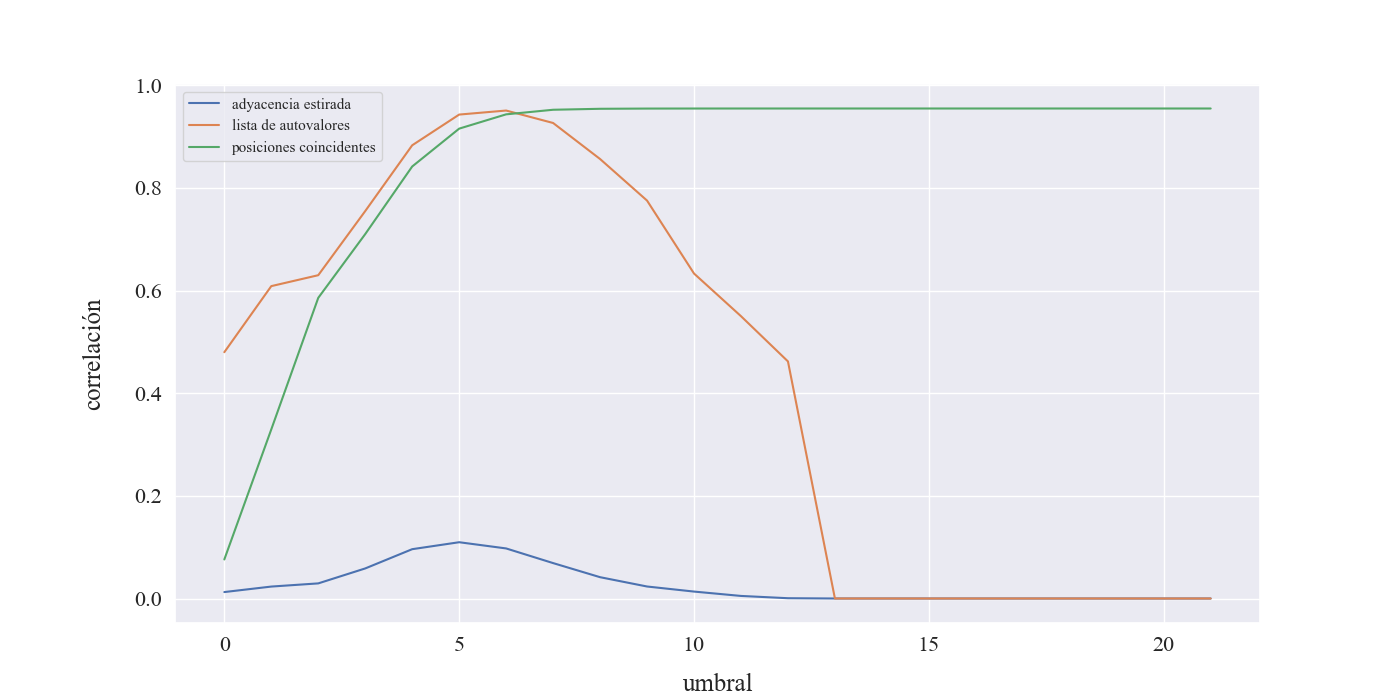
\includegraphics[scale=0.45]{/files/src/.media/ego/facebook_similaridad.png}
\caption{Similitud entre las aproximaciones y el grafo \textbf{E} para \textit{posiciones coincidentes}, \textit{adyacencia estirada} y \textit{lista de autovalores}, en función del umbral $u$.}
\label{grafo_correlaciones}
\end{figure}

\vspace{1em}
¿Cuál es, entonces, el valor para $u$ que genera la mejor aproximación? 
La figura (\ref{grafo_correlaciones}.) permite deducir que los mejores umbrales son $u = 5$ y $u = 6$. Los grafos formados bajo estas condiciones parecerían tener las mejores correlaciones con la red `ego' verdadera, sobre todo al comparar con las aproximaciones de umbrales muy bajos ($u < 2$) o muy altos ($u > 10$). Esto tiene sentido dado que mantienen una cantidad de conexiones similares al grafo original ---característica observable en la figura (\ref{grafos_aproximados}.)---, y los demás umbrales parecerían tener muy pocas aristas (hasta ninguna) o demasiadas.

Sin embargo, notamos que los resultados son considerablemente distintos a la red original. Un análisis más detallado revela que con incluso ambas de las mejores aproximaciones, $u = 5$ y $u = 6$, la cantidad de conexiones acertadas fueron tan solo 2,666 (16.87\%) y 1,106 (7.89\%) respectivamente. Aún más, la cantidad de conexiones sobrantes (existentes en la aproximación pero no en la original) fueron 14,484 y 4,621. En otras palabras, el 85.96\% de las aristas en la aproximación con $u = 5$ y el 80.69\% con $u = 6$ están de más. El método de aproximación por matriz de similaridad propuesto no fue capaz, en nuestra opinión, de capturar la estructura de la red original. 

% \vspace{2em}
% \subsection{Comparación con la red original}

% Nos encontramos con diferentes grafos construidos en base a los atributos en \textbf{C}. Buscamos ahora comparar nuestras aproximaciones con la red original. 

% Un primer acercamiento a este problema puede ser calcular la cantidad de posiciones coincidentes entre las matrices de adyacencia y dividir por los elementos totales. La lógica por detrás del método es que nuestros grafos serán más similares entre sí por cada conexión y `no conexión' acertada. Entonces, por cada 0 y 1 coincidente en nuestra aproximación y \textbf{E} nos acercaríamos más a un 100\% de similitud. 

% % aca creo que quedaria mejor primero mencionar todos los metodos
% % despues mostrar tabla resultados
% % y grafico
% % y despues hacer el analisis

% \begin{figure}[!htbp]
% \begin{equation*}
%     \begin{bmatrix}
%     0  &\%\ 7.6054231  &298.799 \\
%     1  &\%\ 32.947445  &213.902\\
%     2  &\%\ 58.570142   &127.382\\
%     3  &\%\ 70.993985    &86.847\\
%     4  &\%\ 84.162733   &43.091\\
%     5  &\%\ 91.537012   &16.850 \\
%     6  &\%\ 94.322073   &5.727\\
%     7  &\%\ 95.214277   &1.517\\
%     8  &\%\ 95.403337   &405\\
%     9  &\%\ 95.446393   &108 \\
%     10 &\%\ 95.455457   &36\\
%     11 &\%\ 95.458695   &8\\  
%     12 &\%\ 95.459342   &2\\
%     13 &\%\ 95.459990   &0\\
%     \end{bmatrix}
% \end{equation*}
% \caption{Similitud elemento a elemento de las matrices de adyacencia, la primer columna representa el umbral tomado para la aproximación y la segunda el porcentaje de elementos correctamente estimados con respecto a \textbf{E}. La tercera columna indica la cantidad de aristas del grafo; la red `ego' original cuenta con 14.024.} \label{promedio_similaridad}
% \end{figure}

% Como puede observarse en (\ref{promedio_similaridad}.), desafortunadamente, los grafos con muy pocas conexiones, como prueban ser tomando los umbrales $u > 10$, tienen de los valores más altos, mientras que otros con cantidad de aristas similares a la red original, como con $u = 5$ o $u = 6$ (16.850 y 5.727 conexiones respectivamente), parecerían ser peores aproximaciones. Esto se da por la naturaleza rala de nuestras matrices de adyacencia. La de la red `ego' \textbf{E} es de $786 \times 786$, con 617.796 elementos, y tan solo 28.048 (\% 4.54) de ellos son no nulos. Es decir, es rala en un \% 95.46. Es por esto que comparar elemento a elemento no prueba ser un método muy descriptivo de qué tan buena es una aproximación, ya que cualquiera con pocos elementos coincidirá en un $\sim$\% 95.

% \vspace{1em}

% Empleamos entonces otros dos métodos de comparación: \textit{la correlación de las matrices de adyacencia estiradas} y \textit{la correlación de las listas de autovalores}. La correlación es una covarianza normalizada con valores en (-1, 1), donde números mayores indican una mayor similitud. Esta es descrita por la siguiente fórmula:

% \begin{equation}
%     Corr(x, y) = \frac{(x - \mu_{x}) \cdot (y - \mu_{y})}{\sqrt[]{(x - \mu_{x})^{2} \cdot (y - \mu_{y})^{2}}}
% \end{equation}

% siendo $\mu$ el valor medio de los vectores.

% \vspace{1em}
% \begin{figure}[!htbp]
% \centering
% 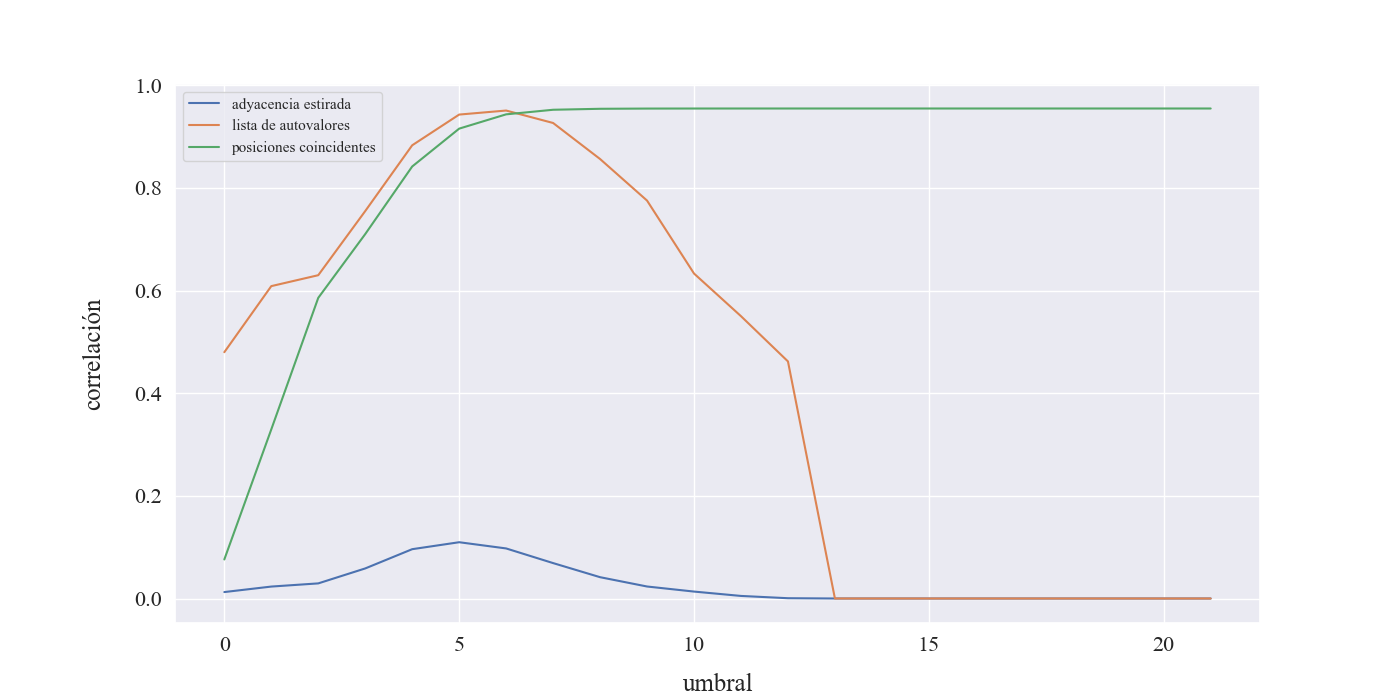
\includegraphics[scale=0.45]{/files/src/.media/ego/facebook_similaridad.png}
% \caption{Correlaciones entre matrices de adyacencia y listas de autovalores según los diferentes umbrales.}
% \label{grafo_correlaciones}
% \end{figure}

% En la figura (\ref{grafo_correlaciones}.) se puede apreciar que se obtienen resultados considerablemente diferentes a los de nuestro primer método de comparación. En un primer lugar, siguiéndonos de la correlación entre las matrices de adyacencia, parecería que las mejores aproximaciones son, razonablemente, las de cantidad de aristas similares a la red original (ver \ref{grafos_aproximados}.), con los umbrales $u \in [4,7]$, mientras que los grafos vacíos con umbrales más altos pasan a tener correlación 0. De la misma forma, analizando con los autovalores se obtienen resultados similares, donde la mayor correlación se halla con los umbrales de valores medios y decae avanzando para los extremos.  


% % === OPTIMIZACION === %

% \vspace{2em}
% \subsection{Optimización}

% ¿Cuál es entonces el valor para $u$ que genera la mejor aproximación? 
% Observando (\ref{grafo_correlaciones}.), se puede deducir que los mejores umbrales son $u = 5$ y $u = 6$. Los grafos formados bajo estas condiciones parecerían tener las mejores correlaciones con la red `ego' verdadera, sobretodo comparándolos con los de umbrales muy bajos ($u < 2$) o muy altos ($u > 10$). Esto tiene sentido dado que mantienen una cantidad de conexiones similares al grafo original, característica observable en (\ref{grafos_aproximados}.), y los demás umbrales parecerían tener muy pocas aristas (hasta ninguna) o demasiadas.


% === PCA === %

\vspace{2em}
\subsection{Análisis de componentes principales}

% Ahora bien, el conjunto describe 319 atributos distintos.
% En cada caso su significado puede variar notablemente.
% Su impacto sobre el sistema de conexiones puede diferir de tal manera que el subconjunto de atributos en consideración
% sea relevante para nuestra exploración del mismo, y tal que parte de los datos sea poco pertinente para dicho estudio.
% El Análisis de Componentes Principales (PCA) es un método que podemos aprovechar para reducir la dimensionalidad de los datos.
% Reduciendo la cantidad bajo consideración podemos obtener un conjunto de atributos que sea más relevante para la exploración del sistema de conexiones.
% PCA proyecta los datos en un espacio de menor dimensionalidad, donde los atributos son linealmente independientes, formando una base de vectores ordenados según su varianza de mayor a menor.
% Es decir, PCA organiza la información según su relevancia. Esto podria eventualmente ayudarnos a reducir la redundacía de los datos, y por ende, la cantidad de atributos que debemos considerar.
% Así se espera intercambiar un poco de precisión, deshaciendonos de información redundante, para ganar simplicidad y eficiencia computacional.

El conjunto \textbf{C} describe 319 atributos distintos, cada uno con un significado diferente\footnote{Si bien los atributos están obfuscados para mantener la privacidad de los usuarios, el dataset permite conocer de manera parcial su significado: existen atributos respecto a fechas de cumpleaños, educación, trabajo, género, nombre, apellido y lugar de residencia; por nombrar algunos. Como cada atributo es binario y múltiples refieren a las mismas cualidades, podemos suponer que no todas las combinaciones son posibles.}. %Por ejemplo, el subconjunto de atributos que designa el nombre es exclusivo dos a dos, por lo que tendrá a lo sumo un bit levantado por usuario.
Su impacto sobre nuestras aproximaciones puede diferir notablemente, de tal manera que es esperable que sólo parte de la información sea relevante para nuestra exploración.

El Análisis de Componentes Principales, \textit{PCA}, es un método que podemos aprovechar para reducir la dimensionalidad de los datos. Si consideramos al conjunto \textbf{C} como una matriz, entonces cada fila designa un usuario y cada columna un atributo. \textit{PCA} nos permite proyectar las columnas de esta matriz a un espacio de menor dimensión donde las columnas son linealmente independientes y están ordenadas según su varianza de mayor a menor.

Es decir, PCA organiza la información según su relevancia. Esto nos ayudará a reducir la redundacía de los datos, y por ende, la cantidad de atributos que debemos considerar. Así se espera intercambiar un poco de precisión, al remover información redundante, para ganar simplicidad y eficiencia computacional.

% Para lograr esto, se busca hacer un cambio de base a la matriz de datos $\textbf{C}$. 
% Y para eso vamos a diagonalizar la matriz de covarianza $\textbf{M}_x$.
% Esta contiene en su diagonal los valores de varianza de cada variable, y la covarianza (definida en \ref{eq:corr}) en el resto de sus 
% posiciones.
% La obtenemos de la siguiente manera:
% Buscamos diagonalizar esta matriz tal que, para $\textbf{M}_x = \textbf{V}\textbf{D}\textbf{V}^t$, $\textbf{V}$ contiene los autovectores de % $\textbf{M}_x$ en sus columnas.
% Permutamos las columnas de $\textbf{V}$ para que estén ordenadas de mayor a menor según los valores de la diagonal de $\textbf{D}$, los % autovalores de $\textbf{M}_x$, y obtenemos $\textbf{V}^*$. 
% La matriz resultante con base cambiada es $\textbf{C}^* = \textbf{C}\textbf{V}^*$.

\vspace{1em}
\noindent Para lograr esto, se buscará hacer un cambio de base a la matriz de datos \textbf{C}. 

\vspace{1em}
La matriz de covarianza \textbf{M}$_x$, contiene en su diagonal los valores de varianza de cada variable, y la covarianza ---definida en (\ref{eq:corr}.)--- en el resto de sus posiciones. % La obtenemos de la siguiente manera:

\vspace{1em}
\begin{equation}
	\mathbf{M}_x = \frac{\mathbf{C}^t \mathbf{C}}{n-1}
\end{equation}

\vspace{1em}
\noindent donde $n$ es la cantidad de nodos en el grafo.

\vspace{1em}
Si diagonalizamos esta matriz, tal que $\mathbf{M}_x = \mathbf{V} \mathbf{D} \mathbf{V}^t$ ---donde \textbf{V} contiene los autovectores de \textbf{M}$_x$ en sus columnas y \textbf{D} sus autovalores---, y permutamos las columnas de $\textbf{V}$ para que estén ordenadas de mayor a menor según sus autovalores asociados, obtendremos el cambio de base buscado:

\vspace{1em}
\begin{equation}
    \mathbf{C}^* = \mathbf{C} \mathbf{V}^*
\end{equation}

\vspace{1em}
\noindent donde $\mathbf{V}^* := \mathbf{V} \mathbf{P}$, con \textbf{P} una matriz de permutación.

% Podemos limitar el subconjunto de componentes principales a considerar.
% Definimos una variable $p$ como el porcentage de componentes que deseamos preservar en nuestro conjunto.

% La totalidad de los resultados obtenidos se adjuntan en el apendice (ver figuras \ref{similaridad_pca} y \ref{similaridad_pca_2}). 
% En la figura \ref{grafo_correlaciones_pca}, ilustramos nuevamente los distintos métodos de comparación para cada iteración de $p$.

\vspace{1em}
Podemos limitar el subconjunto de componentes principales a considerar. Para ello, definimos la variable $p$ como el porcentaje de componentes que deseamos preservar en nuestro conjunto. Es decir, el tamaño de la matriz $\textbf{V}^*$ va a depender de este valor.

% Así procedemos a trabajar con el valor $p$ y el umbral $u$ para estudiar nuevamente la aproximación de $\textbf{E}$. Usando $\textbf{C}^*$ construimos la matriz de similaridad e iteramos sobre el rango de umbrales.

\vspace{1em}
Procederemos a trabajar con el valor $p$ y el umbral $u$ para estudiar nuevamente las aproximaciones de $\textbf{E}$.
Usaremos $\textbf{C}^*$ para construir la matriz de similaridad e iteraremos sobre el rango de umbrales como en la sección anterior.

\vspace{2em}
\noindent \textsc{Resultados}. La totalidad de los resultados obtenidos se adjuntan en el apendice (ver figuras (\ref{similaridad_pca}.) y (\ref{similaridad_pca_2}.)). 
En la figura (\ref{grafo_correlaciones_pca}.) ilustramos nuevamente los distintos métodos de comparación para cada iteración de $p$.
Para los valores de $p$ más pequeños, el grafico difiere notablemente de los obtenidos en la sección anterior. 
Pero vemos que, como es de esperar, los resultando tienden a converger al mismo comportamiento observado previamente.

\begin{figure}[!htbp]
    \centering
    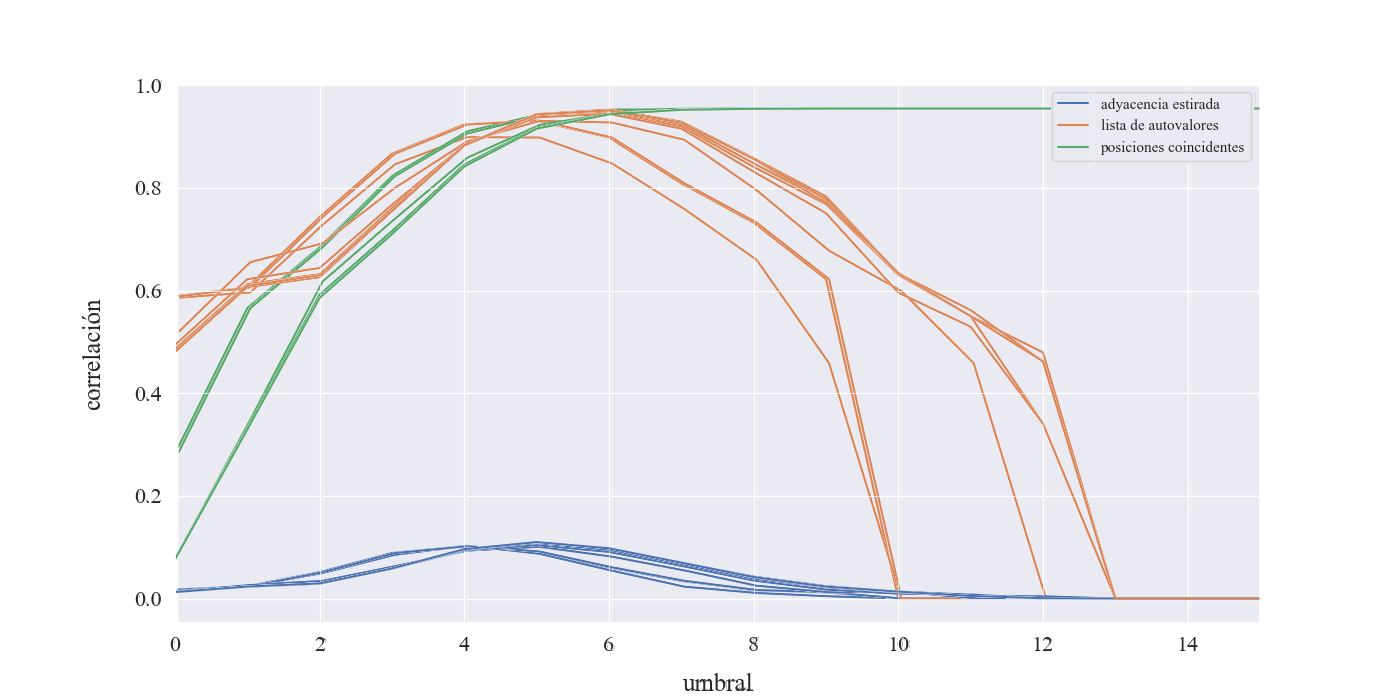
\includegraphics[scale=0.45]{/files/src/.media/ego/facebook_similaridad_pca.png}
    \caption{Similitud entre las aproximaciones y el grafo \textbf{E} para \textit{posiciones coincidentes}, \textit{adyacencia estirada} y \textit{listas de autovalores}, en función del umbral $u$, para todo $p\ \in\ \{0.4, 0.5, 0.6, 0.75, 0.8, 0.85, 0.9, 0.95, 0.99\}$.}
    \label{grafo_correlaciones_pca}
\end{figure}

\vspace{1em}
Lo más interesante es que, con menos atributos, el valor de correlación máximo difiere solo ligeramente.
Y este llega a su tope para un umbral $u$ relativamente menor.
La tabla (\ref{tabla_correlaciones_pca}.) muestra exactamente para qué valor de $u$ se alcanza la máxima correlación, en función del valor de $p$, para los métodos de \textit{adyacencia estirada} y \textit{listas de autovalores}.

\vspace{1em}
\begin{figure}[!htbp]
    \begin{tabular}{ c|c|c|c|c } 
    \hline
     & \multicolumn{2}{c}{adyacencia estirada} & \multicolumn{2}{c}{lista de autovalores} \\
    \hline
    p & u & máximo & u & máximo \\
    \hline
    0.4            &4       &10.29\%                 & 4    &89.88\%  \\
    0.5            &4       &10.18\%             & 5    &93.12\%  \\
    0.6            &5       &10.8\%                & 5     &93.05\%      \\
    0.75            &5      &10.4\%              & 6    &94.42\%     \\
    0.8            &5       &10.49\%             & 6    &94.7\%      \\
    0.85            &5      &10.81\%              & 6       &94.94\% \\
    0.9            &5       &10.96\%             & 6    &95.2\%  \\
    0.95            &5      &10.99\%              & 6      &95.26\% \\
    0.99            &5      &10.99\%               & 6      &95.06\% \\
    \hline
    \end{tabular} \\
    \bigskip
    \caption{Umbral con correlación máxima para los valores de $p$ en los métodos de \textit{adyacencia estirada} y \textit{listas de autovalores}.} \label{tabla_correlaciones_pca}
\end{figure}

% Efectivamente, para menor valores de $p$ empeora nuestra capacidad de aproximar $\textbf{E}$, pero solo levemente.
% Notar que habiendo reducido la cantidad de atributos en un 60\%, perdemos no más que 0.7\% y 5\% en la adyacencia estirada y la lista de autovalores, respectivamente.
Vemos que, para valores de $p$ menores, empeora nuestra capacidad de aproximar $\textbf{E}$, pero solo levemente.
Notamos que habiendo reducido la cantidad de atributos en un 60\%, perdemos no más que el 0.7\% y 5\% de similitud en \textit{la adyacencia estirada} y las \textit{listas de autovalores}, respectivamente.
Es decir, de necesitar el uso del PCA para reducir la dimensionalidad de los datos, los resultados obtenidos sufren meramente una leve pérdida de calidad.
También, constatamos que el rango de umbrales en los que se alcanza la máxima correlación converge a los mismos valores que en la sección anterior.
Es decir, para $u \in \{5, 6\}$.
